\documentclass[10.5pt]{config}
% 本实验报告采用 署名-相同方式共享 4.0 国际许可协议 (CC BY-SA 4.0)
\usepackage{bigstrut,multirow,rotating,booktabs,makecell,array}%表格插件
\usepackage{color, xcolor}

\major{电子科学与技术}
\name{郑智瑄}
\partner{魏希浩} % 签名栏
% \title{}
\stuid{3230103913}
\date{\today}
\lab{东4-216}
\course{电子电路设计实验Ⅱ}
\instructor{叶险峰/施红军/邓靖靖}
\grades{}
\expname{实验设计报告} % 实验名字
\exptype{设计型} % 实验类型

\begin{document}

% \maketitlepage % 封面
% \maketoc % 目录
\makeheader % 首页头部

\section{实验目的}
\begin{enumerate}[leftmargin=2em]
    \item 学习掌握用 Arduino UNO 设计数字时钟;
    \item 学习掌握PCB电路板的设计和制作;
    \item 学习掌握 Arduino UNO 扩展板的设计与制作;
    \item 学习掌握 DS1302 时钟芯片和 LCD1602 液晶显示屏的使用。
\end{enumerate}

\section{实验任务与要求}
\subsection{用 Arduino UNO 设计多功能数字时钟，要求实现功能：}
\begin{itemize}[leftmargin=2em]
    \item 显示时间、日期、星期和温度，并能断电保存时间
    \item 在整点、到达自定义闹钟时间、到达报警温度时报警
    \item 按键功能：按选择键进入设置时间功能；同时按 + - 键进入闹钟和报警温度设置功能；
    \item 再按选择键光标跳动，光标跳到哪，当前的参数即可通过加减键修改
\end{itemize}
\subsection{设计的电路，完成相应器件的选择和参数计算，制作 Arduino UNO 扩展板。}
\subsection{编制与调试多功能数字时钟程序。}
\subsection{将制作的 Arduino UNO 扩展板与 Arduino UNO 板组装后，进行系统联调。}

\clearpage
\section{实验设计方案}
本项目使用 Arduino UNO 设计多功能数字时钟。硬件框图如Figure 1所示，使用出的模块在 Table 1 中列出，下面对各部分模块进行说明。
\begin{figure}[!htbp]
    \centering
    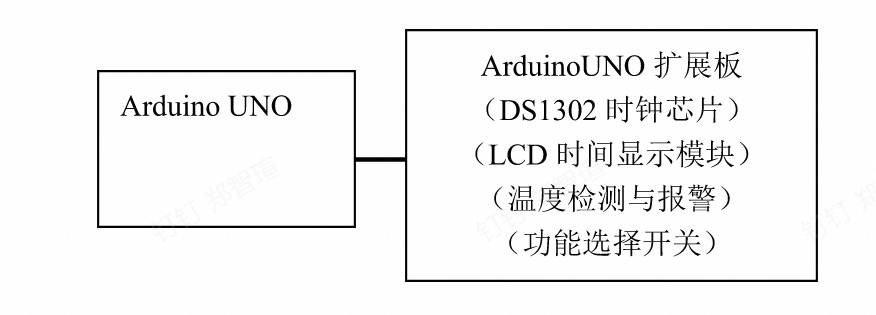
\includegraphics[width=0.8\textwidth]{figures/p1.png}
    \caption{多功能数字时钟框图}
\end{figure}

\begin{table}[H]
  \centering
  
  \label{tab:devices}
  \begin{tabular}{rlp{8cm}}
    \toprule
    编号 & 仪器用具名称 & 备注 \\
    \midrule
    1   & PC 电脑       & 使用 Altium Designer Winter 09 进行设计 \\
    2   & Arduino UNO   & 使用 PlatformIO 进行开发 \\
    3   & DS1302 时钟模块 & 使用 DS1302 库 \\
    4   & LCD1602 液晶显示屏 & 使用 LCD1602 库 \\
    6   & LM35 温度传感器 & -- \\
    5   & 无源蜂鸣器     &  \\
    7   & 按键          & -- \\
    8   & 电阻、排针若干  & -- \\
    \bottomrule
  \end{tabular}
  \caption{实验设备列表}
\end{table}

\subsection{DS1302 时钟芯片}

DS1302 是美国 DALLAS 公司推出的一种高性能、低功耗的实时时钟芯片，附加 31 字节静态 RAM，采用 SPI 三线接口与 CPU 进行同步通信，并可采用突发方式一次传送多个字节的时钟信号和 RAM 数据。实时时钟可提供秒、分、时、日、星期、月和年，一个月小与31 天时可以自动调整，且具有闰年补偿功能。工作电压宽达 2.5～5.5V。采用双电源供电（主电源和备用电源），可设置备用电源充电方式，提供了对后背电源进行涓细电流充电的能力。
\begin{figure}[H]
    \centering
    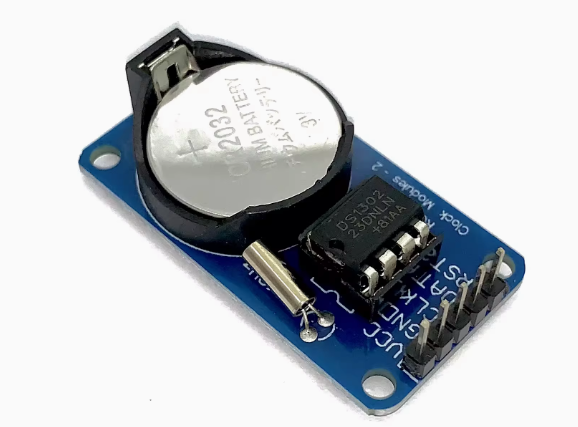
\includegraphics[width=0.3\textwidth]{figures/DS1302.png}
    \caption{DS1032模块图}
\end{figure}

\subsection{LCD 显示模块}

本次实验使用 Arduino UNO 直接驱动 1602 液晶显示字母和数字，LCD 显示模块有一个优势就是将驱动电路集成在模块中。LCD 显示模块具有标准，不同的生产商所生产的大多数模块都可以按相同方法来使用。1602 液晶在应用中非常广泛，最初的 1602 液晶使用的是 HD44780 控制器，现在各个厂家的 1602 模块基本上都是采用了与之兼容的 IC，所以特性上基本都是一致的。
\begin{figure}[H]
    \centering
    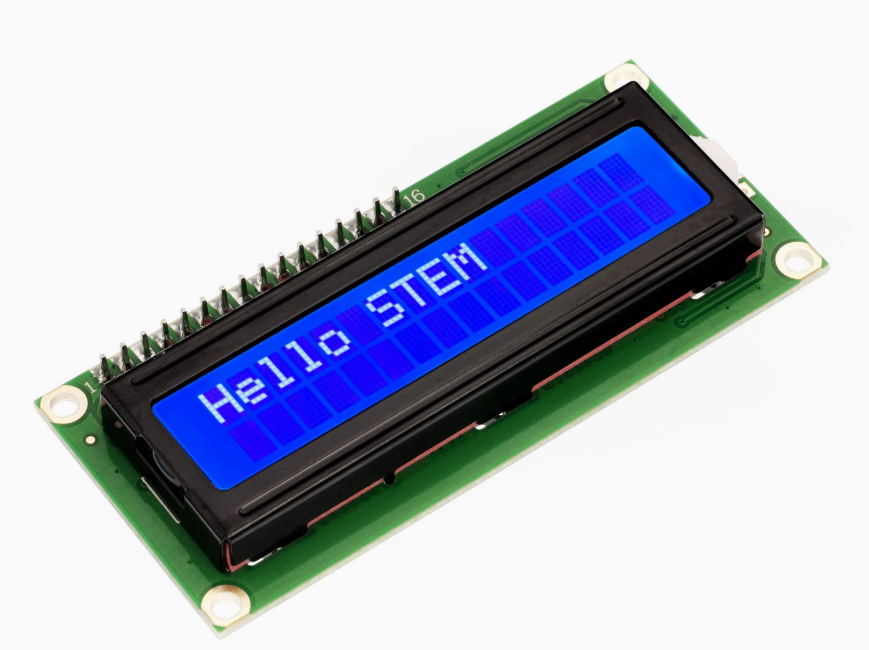
\includegraphics[width=0.3\textwidth]{figures/lcd.png}
    \caption{LCD1602模块图}
\end{figure}

\subsection{温度传感器}

温度传感器可采用 LM35，LM35 是由National Semiconductor 所生产的
温度传感器，其输出电压为摄氏温标。LM35是一种得到广泛使用的温度传感器。
其电源供应模式有单电源与正负双电源两种，其引脚正负双电源的供电模式可提供负温度的量测；两种接法的静止电流-温度关系，在静止温度中自热效应低(0.08℃)，单电源模式在25℃下静止电流约50μA，工作电压较宽，可在4—20V的供电电压范围内正常工作非常省电。
\begin{figure}[H]
    \centering
    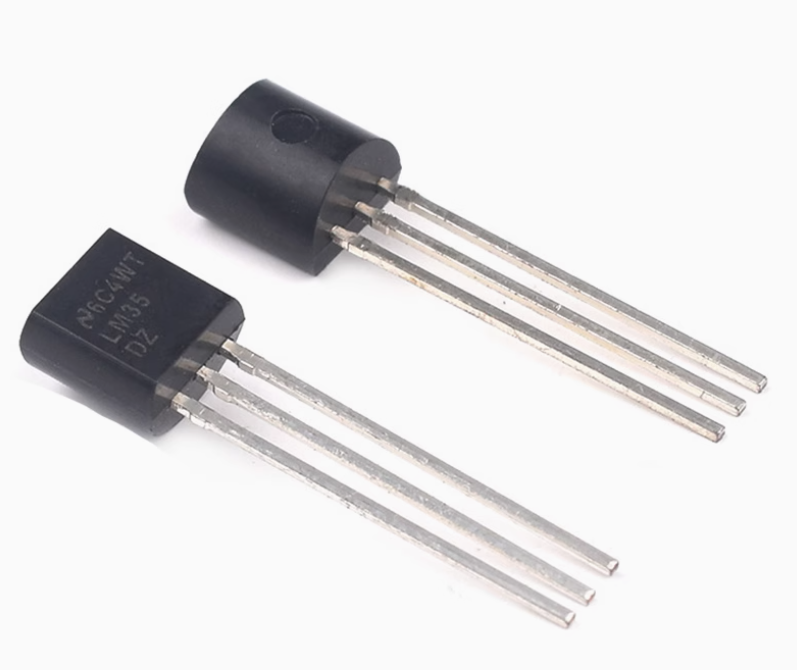
\includegraphics[width=0.3\textwidth]{figures/lm.png}
    \caption{LM35模块图}
\end{figure}

\subsection{无源蜂鸣器}

无源蜂鸣器需要Arduino提供特定频率的脉冲信号，并将方波信号输入谐振装置转换为声音信号输出才能发声，可以通过改变信号频率来调节音调。

\begin{figure}[H]
    \centering
    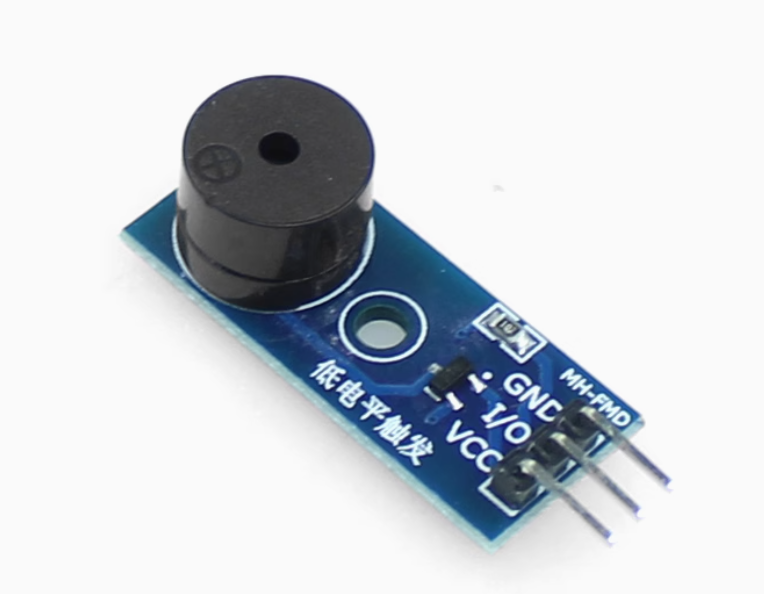
\includegraphics[width=0.3\textwidth]{figures/buzzer.png}
    \caption{无源蜂鸣器模块图}
\end{figure}

\section{硬件设计}
\subsection{参考原理图}
本设计实验主要参考以下设计示例图：
\begin{figure}[H]
    \centering
    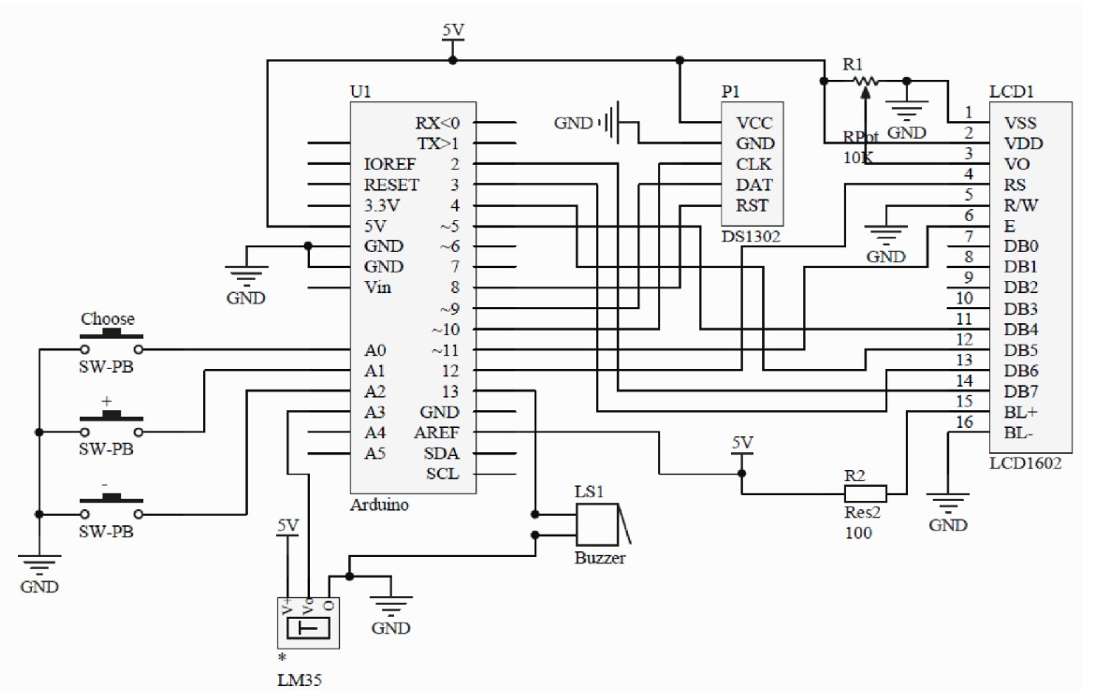
\includegraphics[width=0.6\textwidth]{figures/refer.png}
    \caption{参考原理图}
\end{figure}

\subsection{原理图}
\begin{figure}[H]
    \centering
    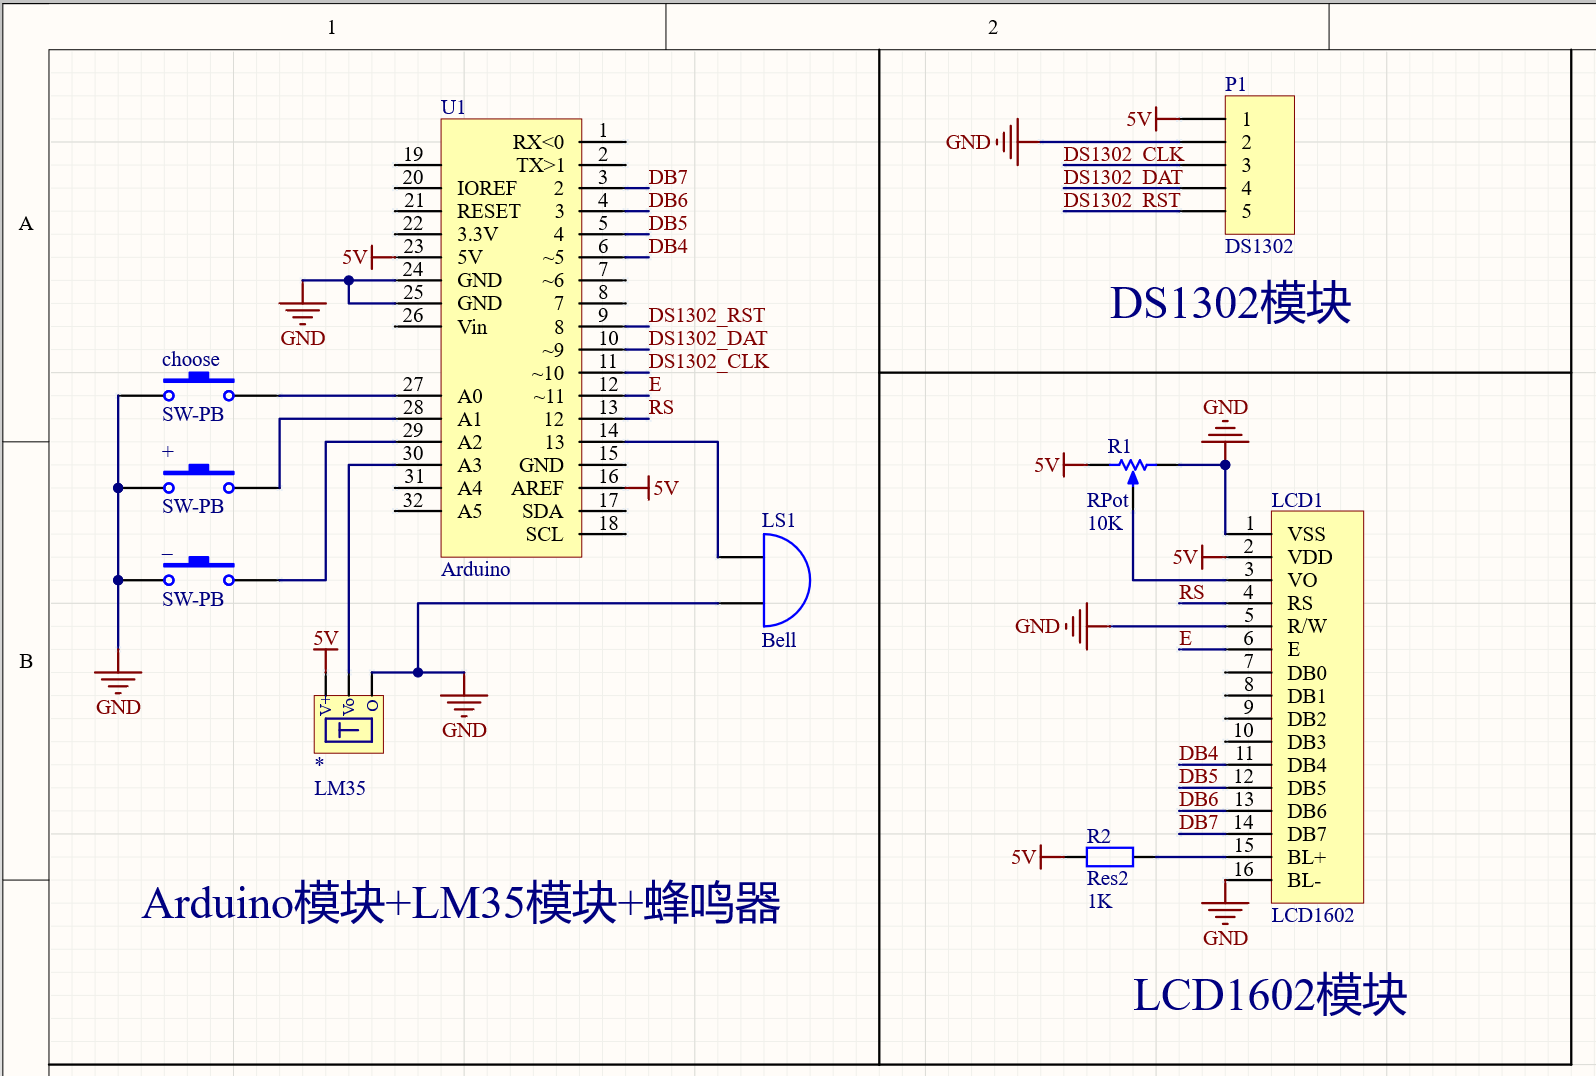
\includegraphics[width=0.6\textwidth]{figures/p2.png}
    \caption{原理图}
\end{figure}

\subsection{PCB图}
\begin{figure}[H]
    \centering
    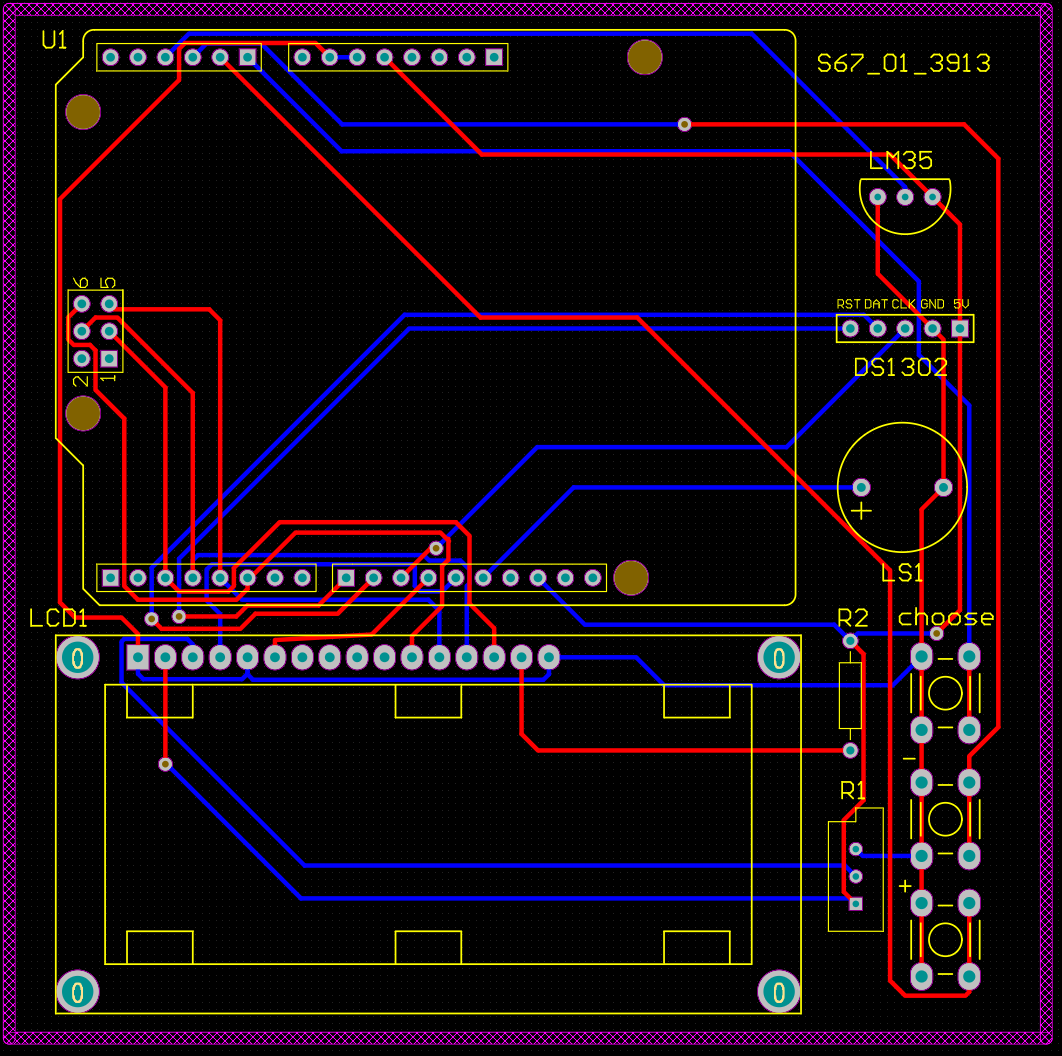
\includegraphics[width=0.6\textwidth]{figures/p3.png}
    \caption{PCB图}
\end{figure}
\clearpage
\subsection{PCB实物图}
\begin{figure}[H]
        \centering
        \begin{minipage}[b]{0.45\linewidth}
            \centering
            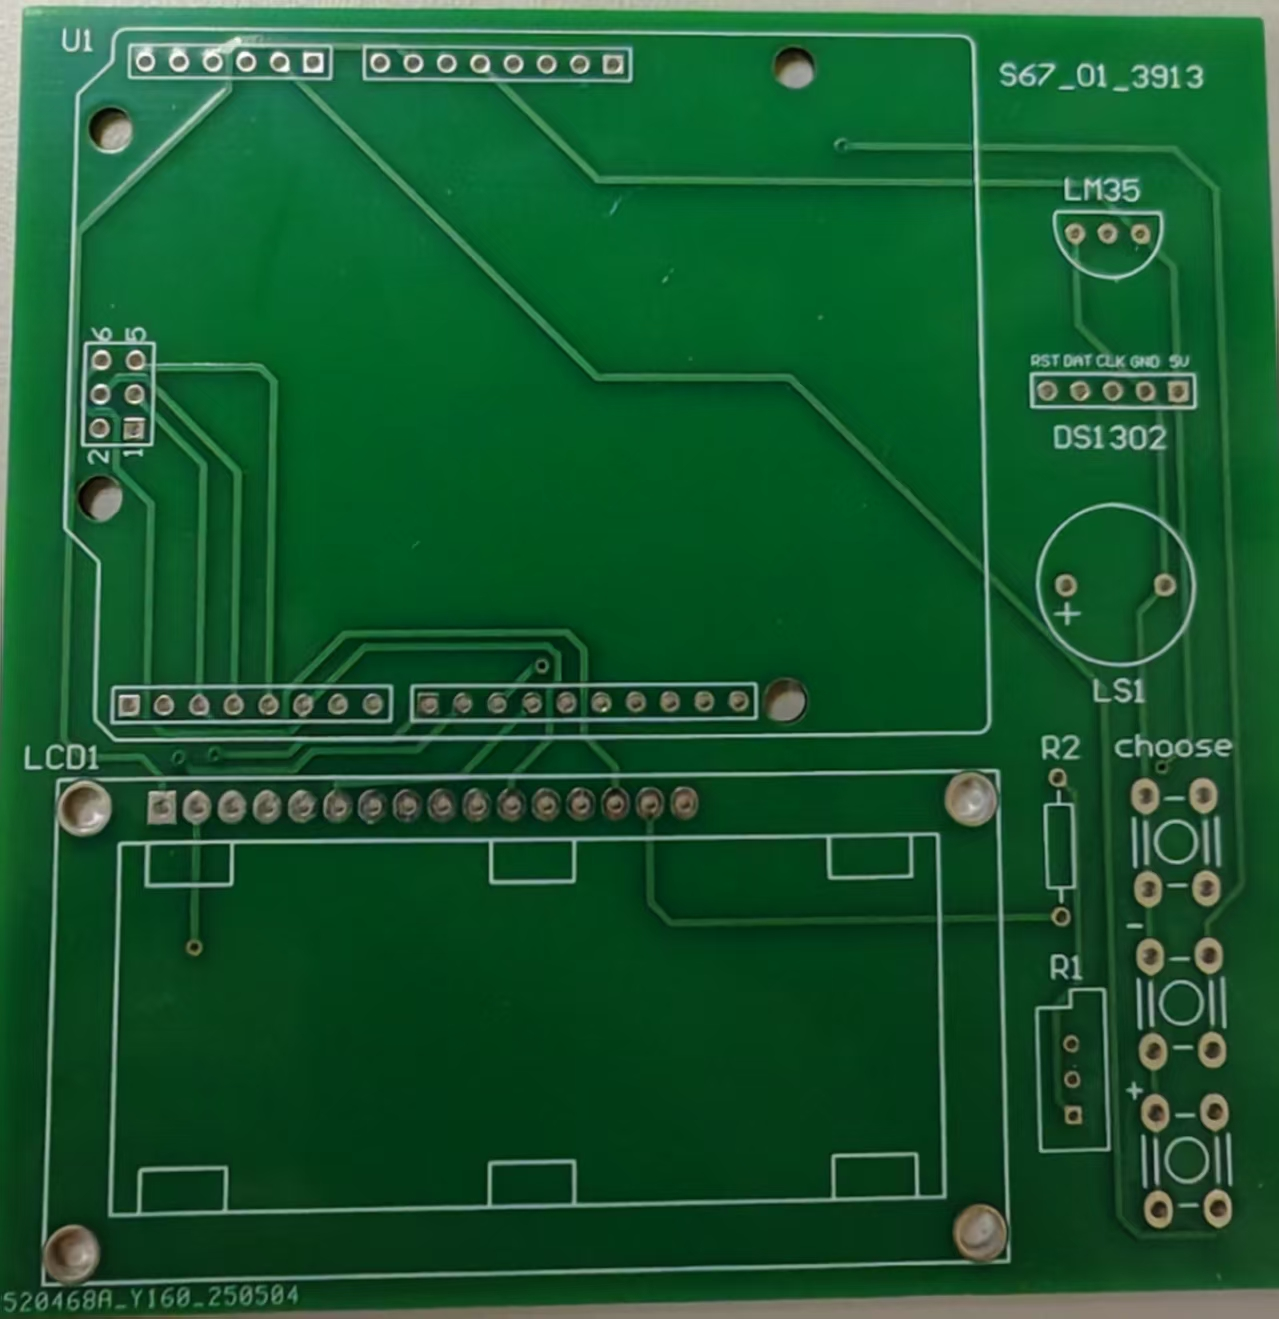
\includegraphics[width=0.9\textwidth]{figures/up.jpg}
            \caption{PCB正面实物图}
            \label{}
        \end{minipage}%
        \begin{minipage}[b]{0.45\linewidth}
            \centering
            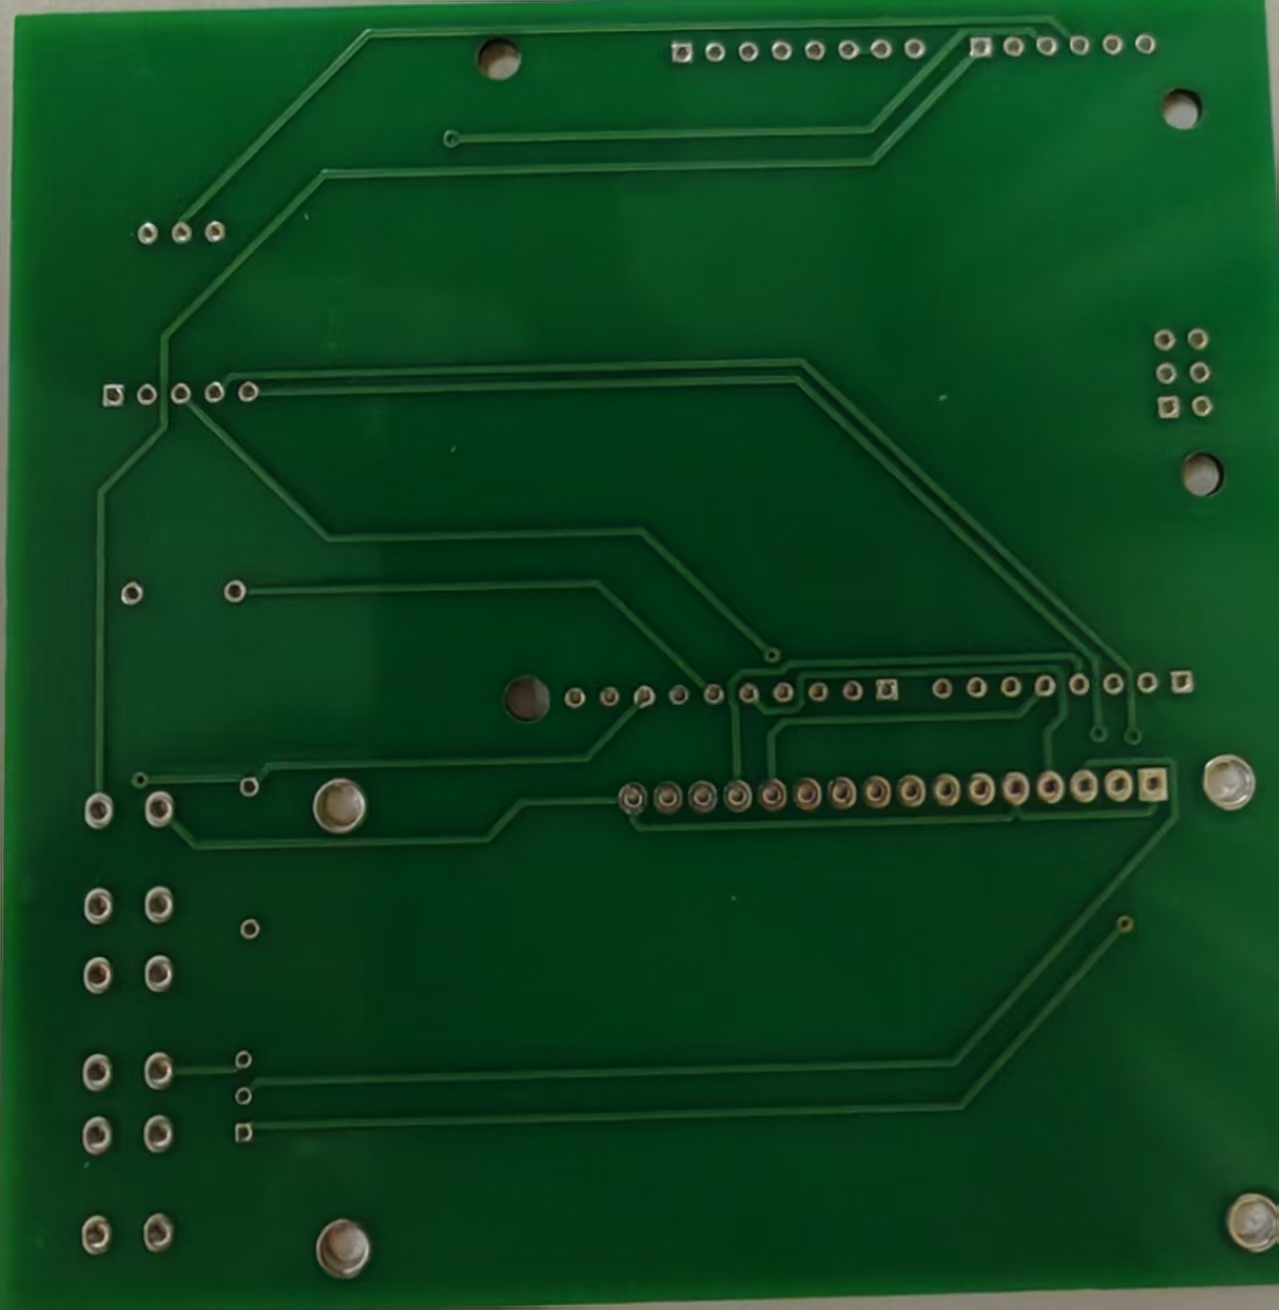
\includegraphics[width=0.9\textwidth]{figures/down.jpg}
            \caption{PCB反面实物图}
            \label{}
        \end{minipage}
    \end{figure}
\section{软件设计}
\subsection{接线设计}
\begin{table}[H]
  \centering
  \begin{tabular}{ll}
    \toprule
    模块 & 接线关系 \\
    \midrule
    \multirow{8}{*}{LCD1602} 
      & VSS → GND \\
      & VDD → 5V \\
      & RS → UNO.12 \\
      & R/W → GND \\
      & E → UNO.11 \\
      & DB4 → UNO.5 \\
      & DB5 → UNO.4 \\
      & DB6 → UNO.3 \\
      & DB7 → UNO.2 \\
    \midrule
    \multirow{3}{*}{按键} 
      & Choose → UNO.A0 \\
      & + → UNO.A1 \\
      & - → UNO.A2 \\
    \midrule
    \multirow{3}{*}{DS1302} 
      & CLK → UNO.10 \\
      & DAT → UNO.9 \\
      & RST → UNO.8 \\
    \midrule
    \multirow{1}{*}{LM35} 
      & Vo → UNO.A3 \\
    \midrule
    \multirow{1}{*}{蜂鸣器} 
      & Buzzer → UNO.13 \\
    \bottomrule
  \end{tabular}
  \caption{接线关系表}
\end{table}

\subsection{代码设计}
\subsubsection{闹钟报警优化}
在所给程序的基础上，我们进行了优化，首先，我们加入了ToneConfig.h文件，保存浙大校歌《大不自多》的音符数据，
以下是ToneConfig.h文件的主要内容：
\begin{lstlisting}[language=C++, caption=Arduino数字时钟音符配置文件]
#ifndef TONE_CONFIG_H
#define TONE_CONFIG_H

#define NOTE_B0  31
#define NOTE_C1  33
#define NOTE_CS1 35
/* 省略部分宏定义 */
#define NOTE_D8  4699
#define NOTE_DS8 4978
#define REST     0

// 每个音符持续时间宏(毫秒)
#define BASE_DURATION 250

const int zheDaSong[] = {
  NOTE_E5, NOTE_E5, NOTE_E5, 
  NOTE_G5, NOTE_C5, 
  NOTE_D5, NOTE_F5, 
  /* 后续省略 */
};

// 每个音符持续时间(毫秒)
const int noteDurations[] = {
  BASE_DURATION*2, BASE_DURATION*2, BASE_DURATION*2, 
  BASE_DURATION*4, BASE_DURATION*2, 
  BASE_DURATION*4, BASE_DURATION*2,
  /* 后续省略 */
};

// 音乐长度
const int songLength = sizeof(zheDaSong) / sizeof(int);

#endif
\end{lstlisting}

\clearpage
其次，我们优化了原有的闹钟报警代码，使其非阻塞式运行，避免了在播放音符时阻塞主循环，从而使得其他功能（如温度检测、时间显示等）可以正常运行。以下是优化后的代码片段：

\begin{lstlisting}[language=C++, caption=Arduino数字时钟报警优化]
// 闹钟音乐控制变量
bool alarmActive = false;          // 闹钟是否激活
int currentNoteIndex = 0;          // 当前播放的音符索引
unsigned long lastNoteTime = 0;    // 上次音符切换的时间
unsigned long currentNoteDuration; // 当前音符持续时间

/** 正点蜂鸣（非阻塞）*/
void Point_Time_Alarm(){
  if(minute == 0 && second == 0 && !hourAlarmActive && !alarmActive) {
    // 激活整点报时
    hourAlarmActive = true;
    hourAlarmStartTime = millis();
    alarmActive = true;
    currentNoteIndex = 1;
    lastNoteTime = millis();
    currentNoteDuration = noteDurations[0];
    isPlayingTone = true;
    if (zheDaSong[0] != REST) {
      tone(Tone, zheDaSong[0]);
    }
  }
}

/** 闹钟指定时间蜂鸣（非阻塞） 与前类似，省略*/
/** 超过指定温度报警（非阻塞） 与前类似，省略 */

void playZheDaSong() {
  unsigned long currentTime = millis();
  
  // 如果没有激活报警，直接返回
  if (!alarmActive) {
    return;
  }
  
  if (screenOff && alarmActive) {
    turnOnScreen();
  }

  // 检查当前音符是否已经播放足够长的时间
  if (isPlayingTone && currentTime - lastNoteTime >= currentNoteDuration - noteSpacing) {
    // 音符播放完毕，进入静音间隔
    noTone(Tone);
    isPlayingTone = false;
    lastNoteTime = currentTime;
  }
  else if (!isPlayingTone && currentTime - lastNoteTime >= noteSpacing) {
    // 静音间隔结束，播放下一个音符
    isPlayingTone = true;
    
    // 移动到下一个音符
    if (currentNoteIndex < songLength) {
      // 如果是休止符，保持静音
      if (zheDaSong[currentNoteIndex] != REST) {
        tone(Tone, zheDaSong[currentNoteIndex]);
      }
      
      // 设置音符持续时间
      currentNoteDuration = noteDurations[currentNoteIndex];
      lastNoteTime = currentTime;
      currentNoteIndex++;
    } else {
      // 播放完毕，重置变量
      alarmActive = false;
      currentNoteIndex = 0;
      isPlayingTone = true;
      noTone(Tone);
    }
  }
}
\end{lstlisting}
\clearpage
\subsubsection{熄屏省电优化}
在实际生活中，功率是一个需要关注的问题，所以我们设计了一个电子钟熄屏省电模式功能。
当设备长时间不使用时，电子钟会自动进入省电模式，这能够有效降低电子钟的功耗。

在省电状态下，系统会关闭LCD的显示，可以减少在不需要频繁查看时间时的能源浪费。
在省电模式下，电子钟仍能进行报警，同时通过简单的按键触碰操作可以随时恢复到正常工作模式，
以下是省电模式的实现代码：
\begin{lstlisting}[language=C++, caption=Arduino数字时钟省电优化]
// 熄屏省电模式变量
unsigned long lastActionTime = 0;    // 上次操作时间
bool screenOff = false;              // 屏幕状态
const unsigned long SCREEN_TIMEOUT = 10000;  // 屏幕超时时间(10秒)

/** 熄屏省电模式 */
void turnOffScreen() {
  if (!screenOff) {
    lcd.noDisplay();                 // 关闭LCD显示
    screenOff = true;
    noTone(Tone);                    // 停止蜂鸣器
    // 保留闹钟功能，但暂时不播放音乐
  }
}

/** 唤醒屏幕 */
void turnOnScreen() {
  if (screenOff) {
    lcd.display();                   // 重新开启LCD显示
    screenOff = false;
    lastActionTime = millis();       // 重置操作时间
  }
}

/** 更新用户操作时间 */
void updateActionTime() {
  lastActionTime = millis();
  turnOnScreen();  // 如果屏幕关闭，则唤醒屏幕
}
\end{lstlisting}
\clearpage
\section{调试}
\subsection{元器件安放问题}
在调试时，我们首先发现，LCD1602的实物比PCB上显示的封装要大，但此时电位器已经焊接上，所以只能采取调一下电位器，插一下LCD1602的方法来调节字符的明暗对比度，比较麻烦
\begin{figure}[H]
    \centering
    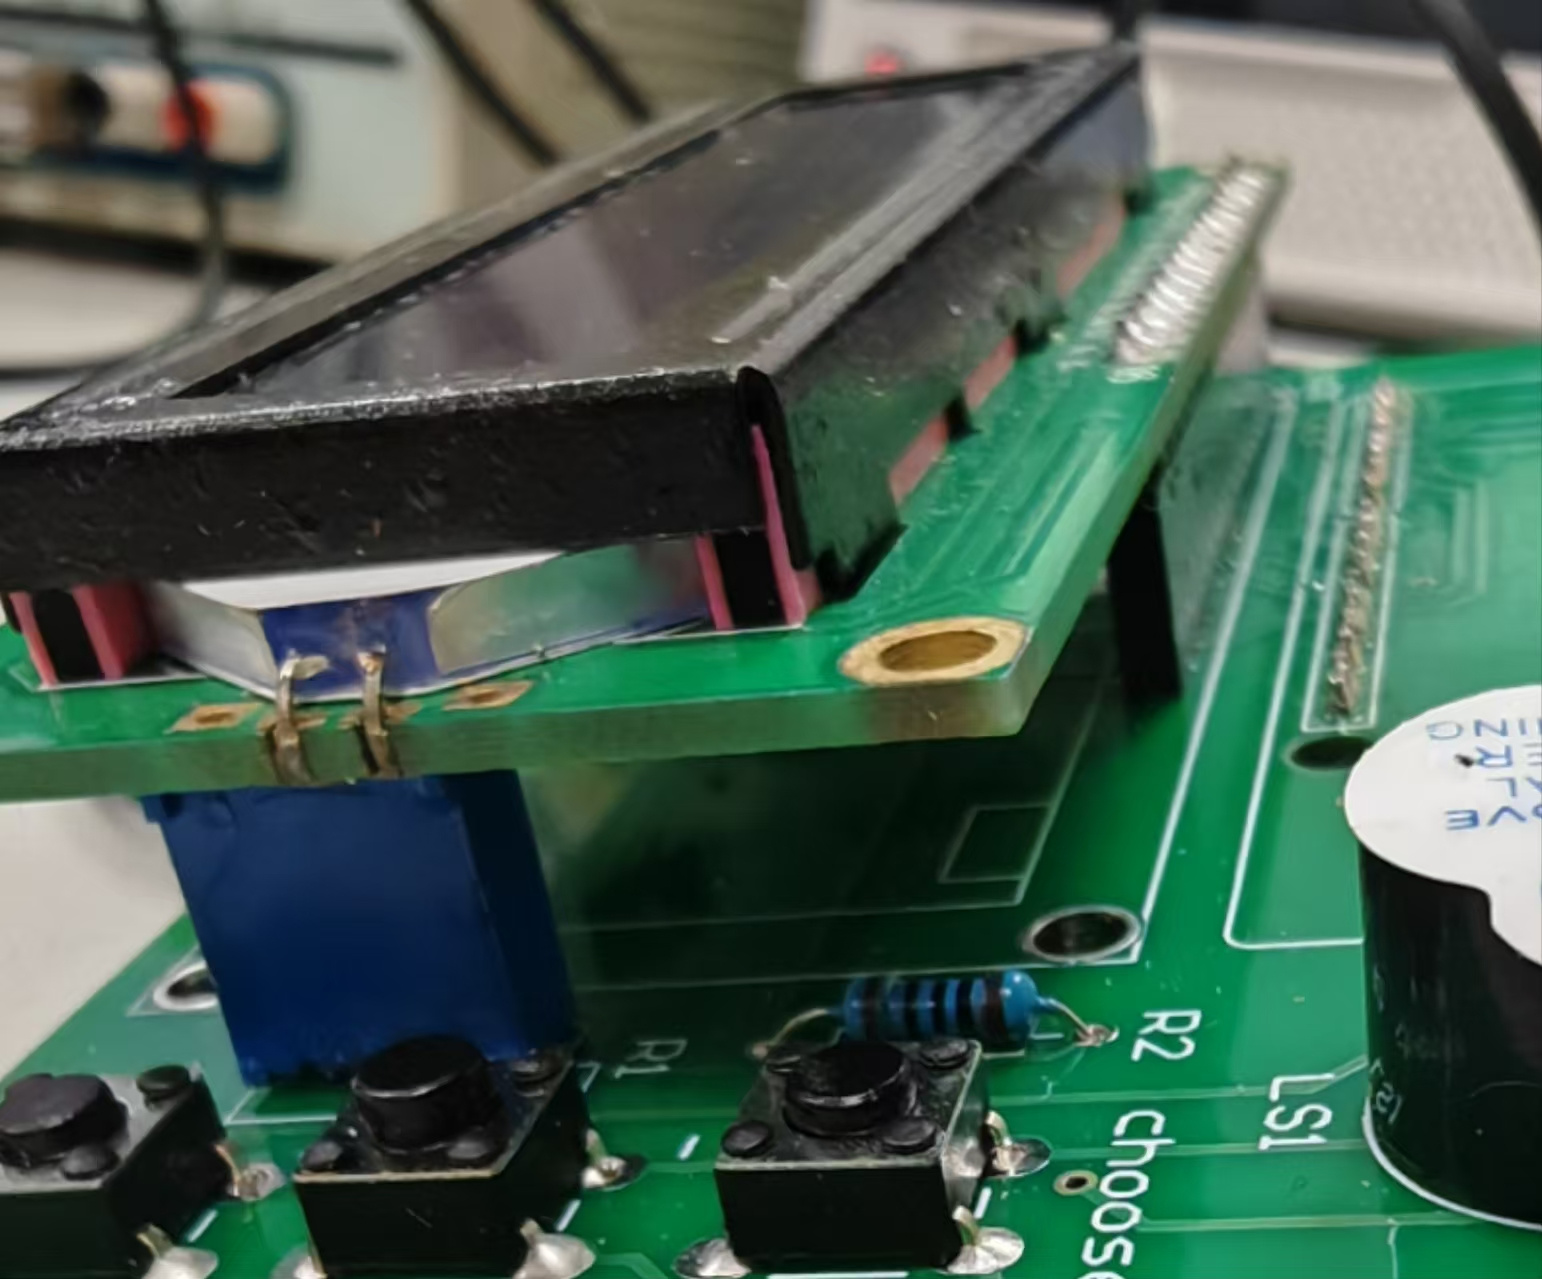
\includegraphics[width=0.45\textwidth]{figures/prob1.jpg}
    \caption{元器件安放问题示意图}
\end{figure}
在继续调试时，我们发现，蜂鸣器不能发声，经过排查，发现不是软件问题，后续发现
是蜂鸣器的正口接上Arduino板子的插线外缘，被强制接地导致不能发声，后续采取
垫一张小纸片进行隔离，成功解决
\begin{figure}[H]
    \centering
    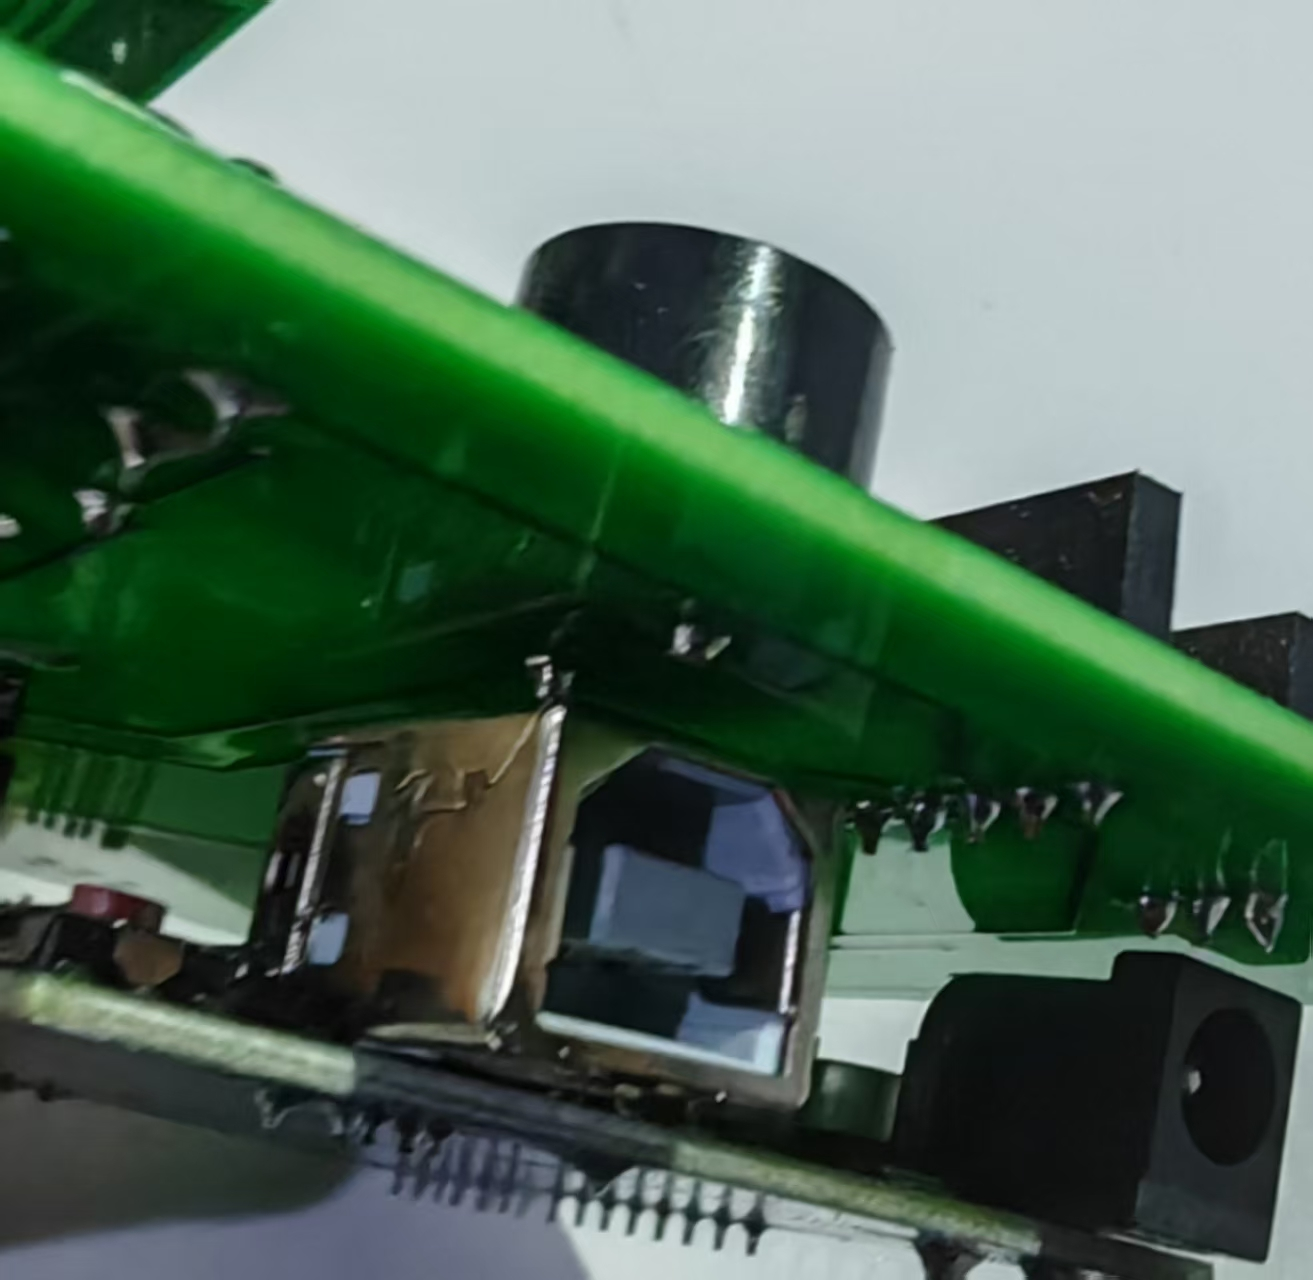
\includegraphics[width=0.45\textwidth]{figures/prob2.jpg}
    \caption{元器件安放问题示意图}
\end{figure}
【总结】：以后需要吸取经验，在设计PCB时要注意实物的大小与点位，防止以上现象的发生。

\subsection{闹钟阻塞运行问题}
我们发现初始的Clock\_ALram函数里使用了delay函数来控制响铃时间，
这种阻塞式运行方法会使得其他功能无法正常运行，所以我们采取了类似中断触发的方法：
在每次循环中检查当前时间是否到达闹钟时间，如果到达，则置布尔变量alarmActive为true
以模拟中断开始，
并在播放音乐时不使用delay函数，而是使用millis()函数来控制音符的播放时间，
这样可以使得其他功能（如温度检测、时间显示等）可以正常运行。

同时，经过如此处理，可以便捷的使用接口函数stopAlarm()来实现按下按钮即停止闹钟响铃。
类似的，我们更改了Point\_Time\_Alarm()与Temperatures\_Alarm()函数，不在此一一列出
\begin{lstlisting}[language=C++, caption=Arduino数字时钟闹钟阻塞运行处理]
void Clock_Alarm(){
  if(hour == alarm_hour && minute == alarm_minute && second == alarm_second && !alarmActive) {
    // 激活闹钟
    alarmActive = true;
    /* 省略其他代码 */
    }
}

void playZheDaSong() {
  unsigned long currentTime = millis();
  
  /* 省略其他代码 */
  else if (!isPlayingTone && currentTime - lastNoteTime >= noteSpacing) {
    // 静音间隔结束，播放下一个音符
    isPlayingTone = true;
  }
  /* 省略其他代码 */
}

void stopAlarm() {
  alarmActive = false;
  /* 省略其他代码 */  
  noTone(Tone);
}
\end{lstlisting}

\section{功能实现}
\subsection{显示时间、日期、星期和温度}
\begin{figure}[H]
    \centering
    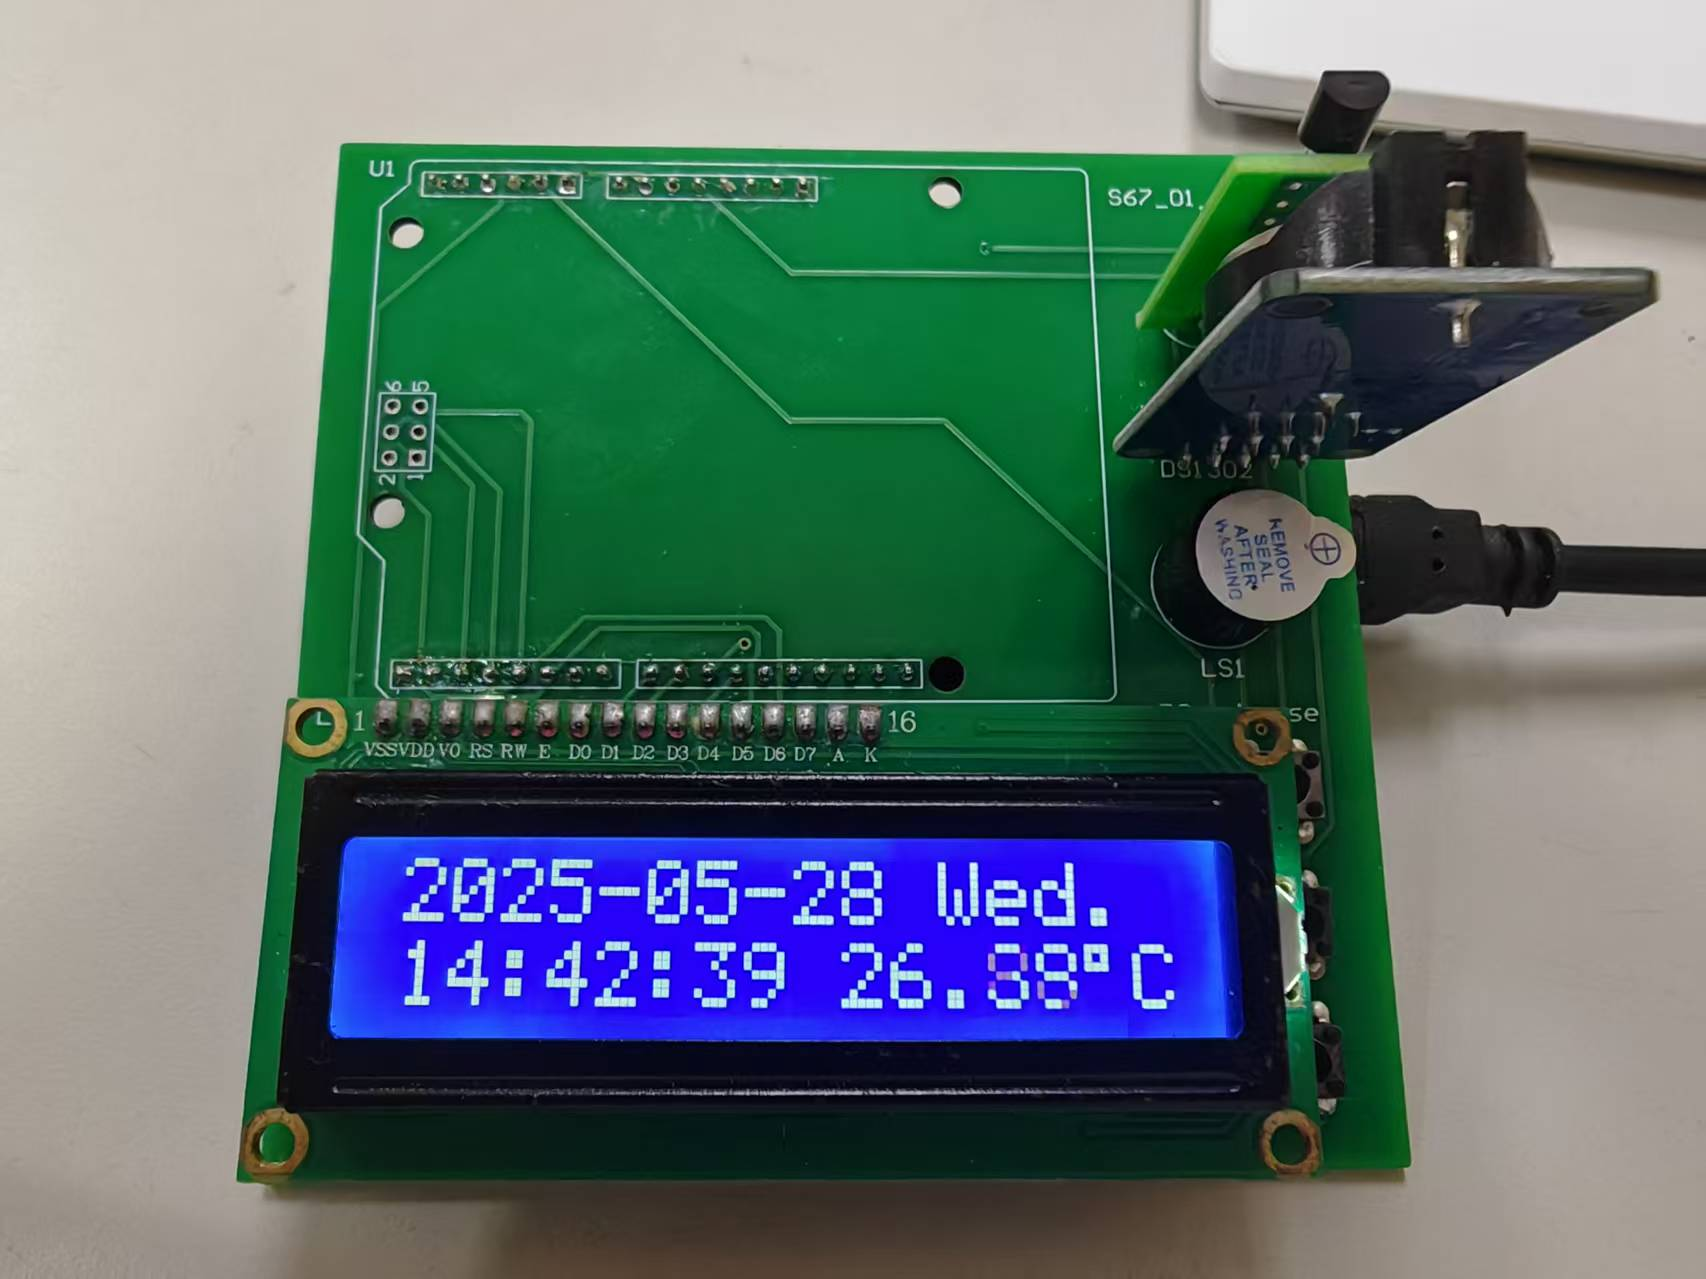
\includegraphics[width=0.5\textwidth]{figures/show1.jpg}
    \caption{显示时间、日期、星期和温度示意图}
\end{figure}
\subsection{按下choose按键显示光标进入设置时间模式}
\begin{figure}[H]
    \centering
    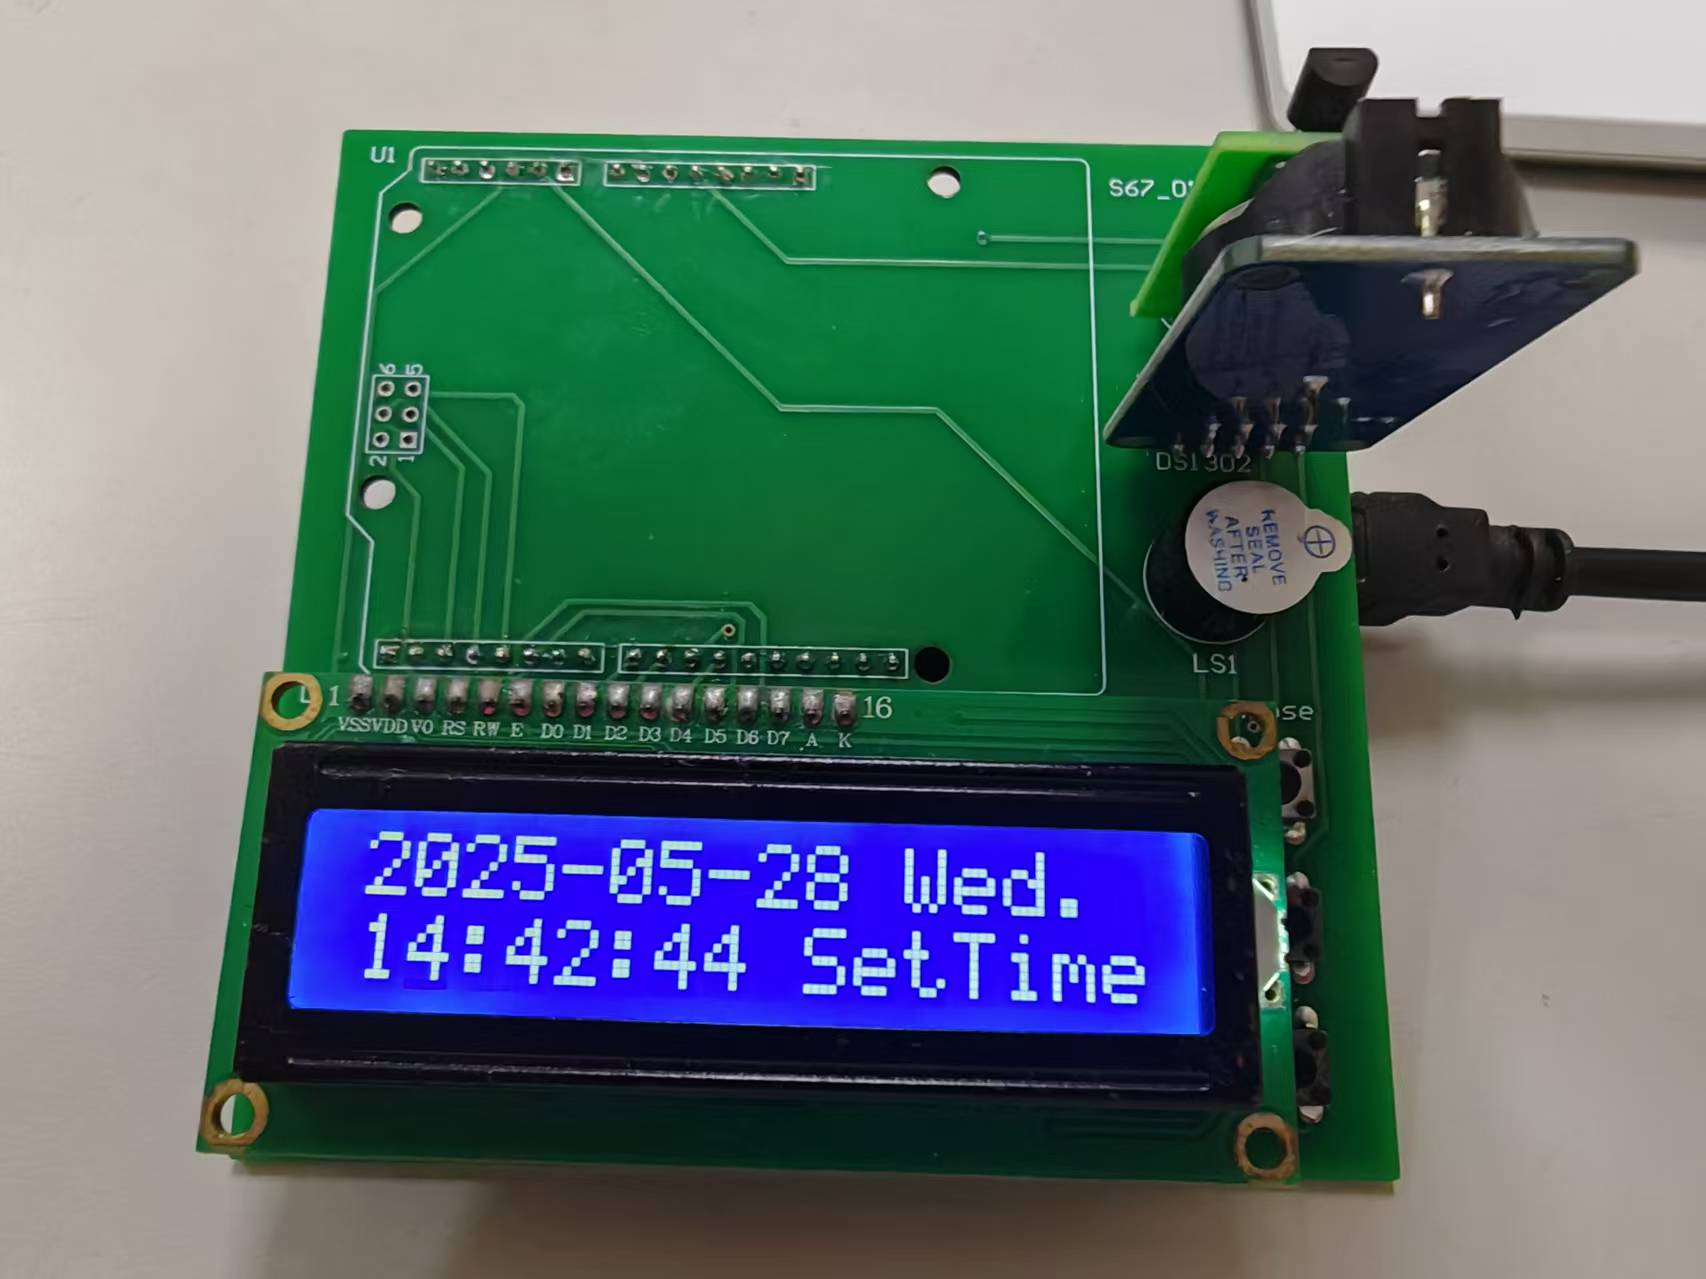
\includegraphics[width=0.5\textwidth]{figures/show2.jpg}
    \caption{显示时间、日期、星期和温度示意图}
\end{figure}
\subsection{同时按下“-”和“+”进入设置闹钟和报警温度模式}
\begin{figure}[H]
    \centering
    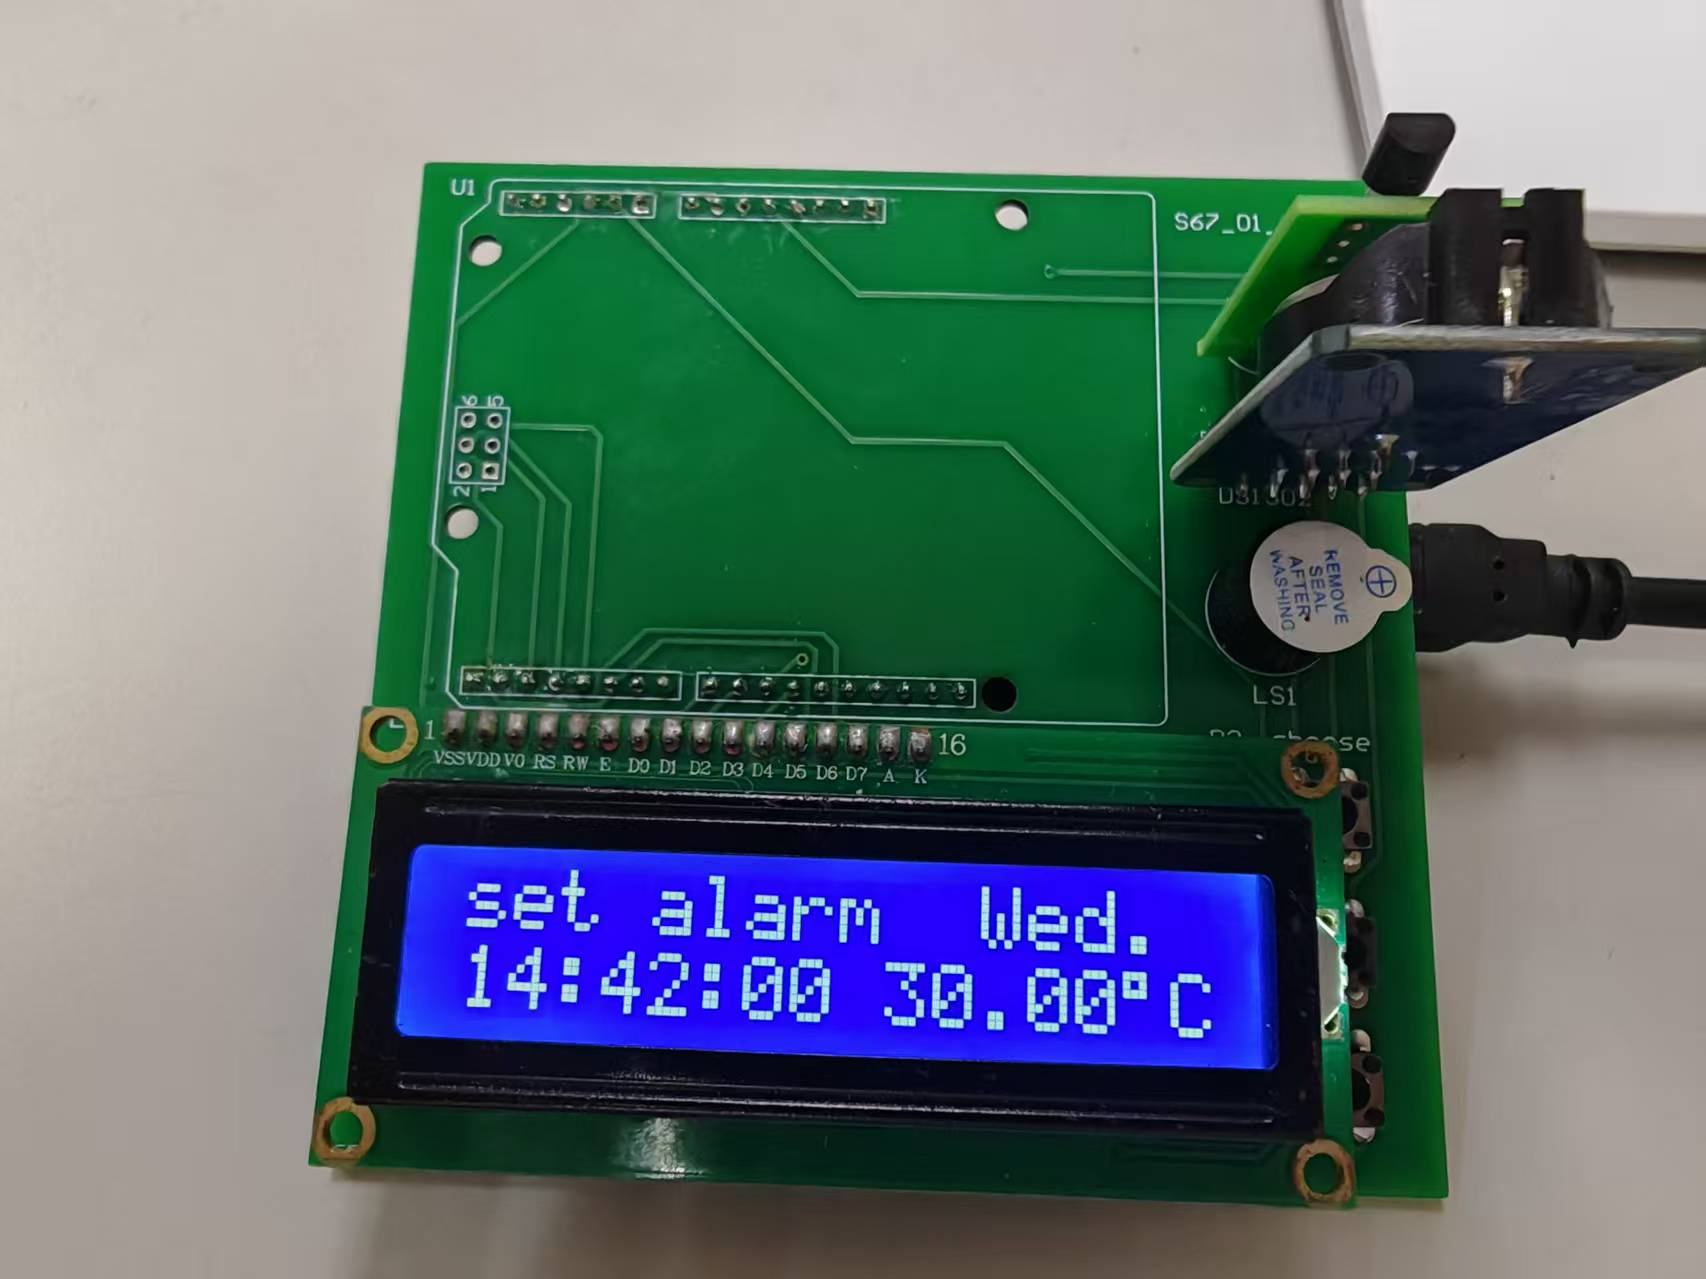
\includegraphics[width=0.5\textwidth]{figures/show3.jpg}
    \caption{按下“-”和“+”进入设置闹钟和报警温度模式示意图}
\end{figure}
\subsection{长时间未使用息屏功能}
  长时间不使用会进行熄屏，实现省电的目标，息屏状态下按任意按钮即可恢复显示
\begin{figure}[H]
    \centering
    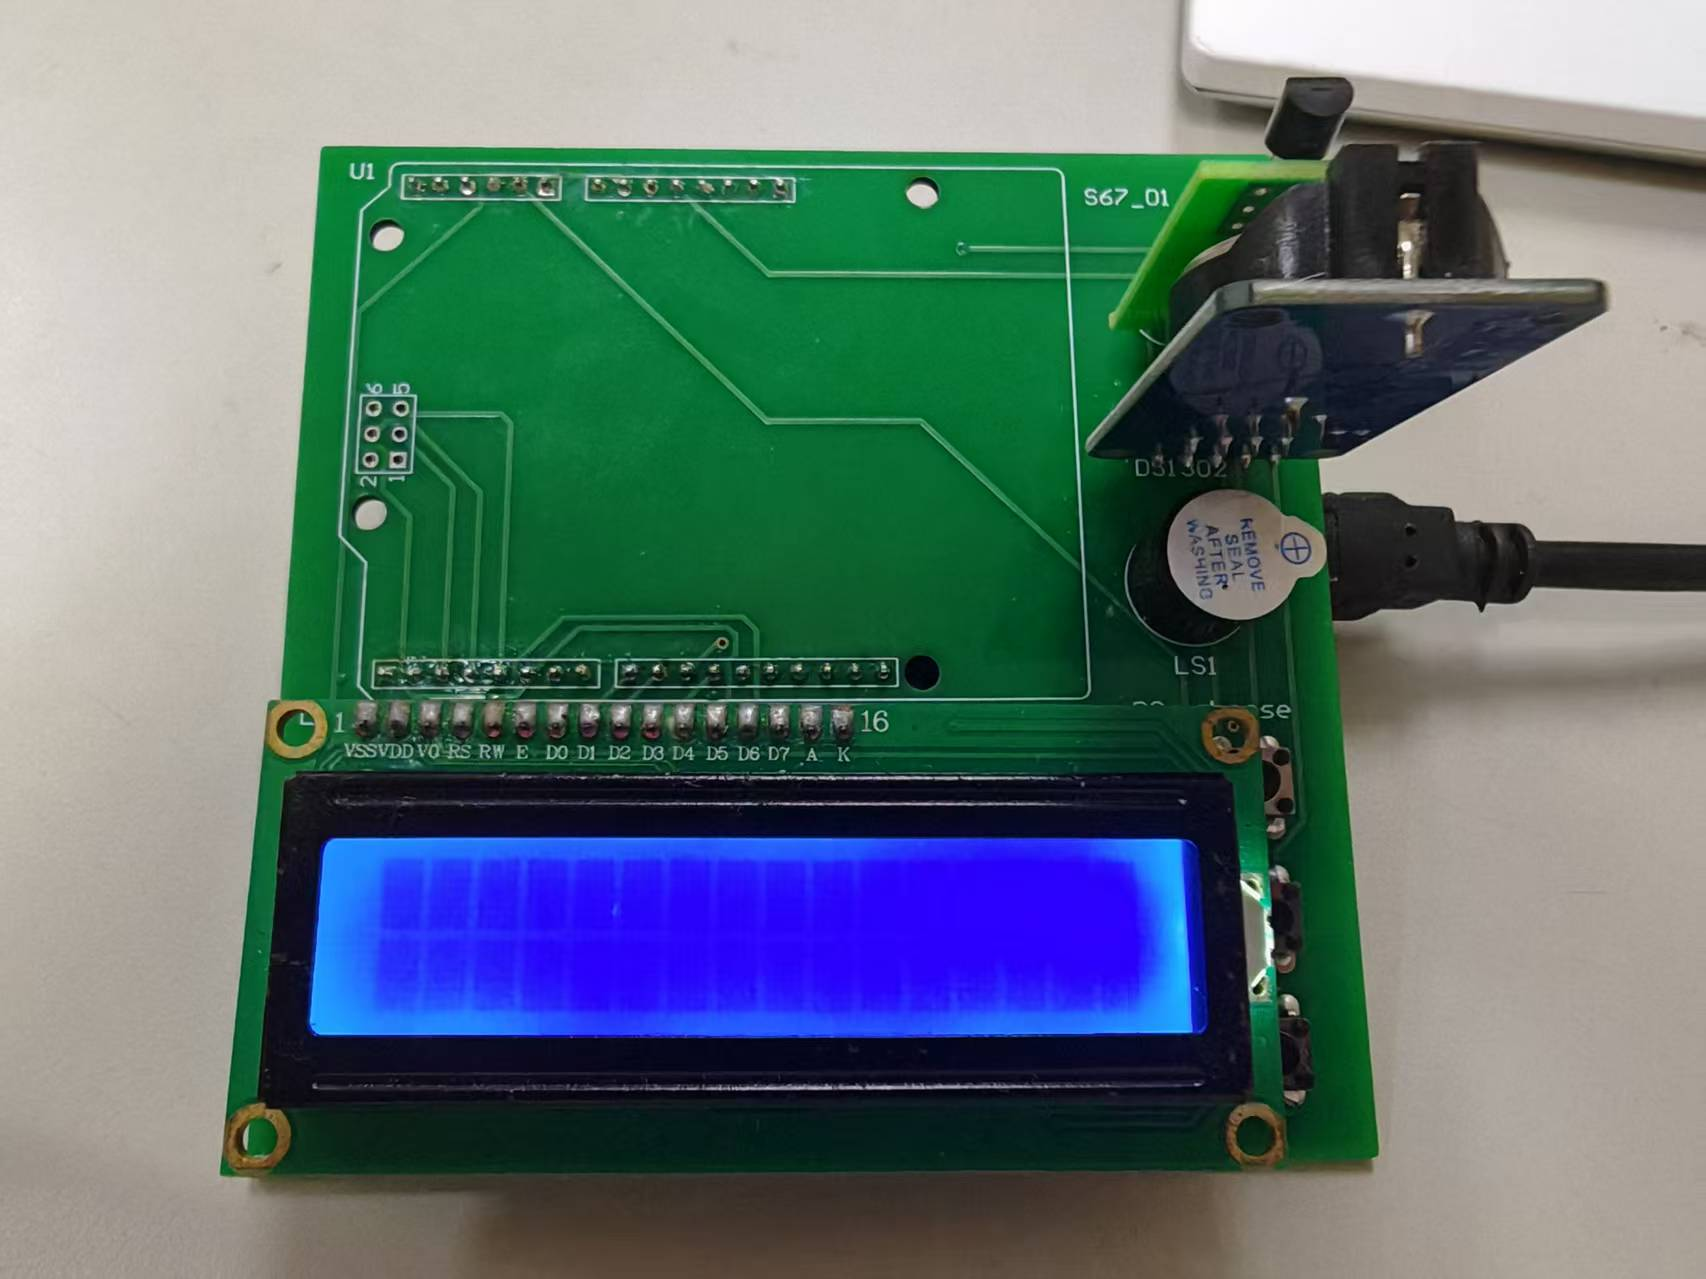
\includegraphics[width=0.5\textwidth]{figures/show4.jpg}
    \caption{长时间未使用息屏功能示意图}
\end{figure}
\subsection{播放/停止音乐功能}
：当高于报警温度/到闹钟设定时间/整点时，播放浙大校歌，并且实现了按下任意键后音乐停止

\section{实验总结与心得}
\subsection{实验总结}

通过本次Arduino多功能数字时钟的设计与实现，我全面掌握了嵌入式系统开发的完整流程,获得了多种能力的提升：

\subsubsection{硬件设计能力}
成功设计并制作了Arduino扩展板，
实现DS1302时钟模块、LCD1602显示屏、LM35温度传感器等关键元件的集成

\subsubsection{软件编程突破}
实现非阻塞式报警系统（整点报时、闹钟、温度报警）
创新开发省电模式（自动熄屏+按键唤醒）
完成浙大校歌《大不自多》的音乐编解码与播放

\subsubsection{系统调试经验}
排查出了LCD尺寸不匹配、蜂鸣器接地异常等硬件问题

\subsubsection{小结}
通过这一系列密集且细致的实践，我掌握了如何将抽象的电路原理转化为可实际加工和测试的PCB版图，并在过程中深刻理解了诸多设计原则的实际应用。这种经历不仅增强了我的工程实践能力，也为我今后在电子工程领域的专业发展奠定了坚实基础。未来，我将以更加系统化、专业化的视角应对各类电路设计挑战，不断提升自身的技术水平与创新能力。
\subsection{实验心得}
在本次实验中，我深刻体会到了电子电路设计的复杂性和挑战性。通过实际操作，我不仅巩固了之前学过的理论知识，还学会了如何将这些知识应用到实际的电路设计中。
在设计过程中，我遇到了许多问题，比如元器件的选择、PCB布局的优化等，这些都需要我不断地学习和尝试。通过查阅资料和请教老师，我逐渐克服了这些困难，完成了实验任务。

总的来说，这次实验让我对电子电路设计有了更深入的理解，也提高了我的动手能力和解决问题的能力。我认识到，电子电路设计不仅仅是一个技术活，更是一个需要创造力和耐心的过程。未来，我希望能在这个领域继续学习和探索，不断提升自己的专业技能。
\clearpage
\section{完整代码}
\begin{lstlisting}[language=C++, caption="ToneConfig.h"]
#ifndef TONE_CONFIG_H
#define TONE_CONFIG_H

// 音符频率定义
#define NOTE_B0  31
#define NOTE_C1  33
#define NOTE_CS1 35
#define NOTE_D1  37
#define NOTE_DS1 39
#define NOTE_E1  41
#define NOTE_F1  44
#define NOTE_FS1 46
#define NOTE_G1  49
#define NOTE_GS1 52
#define NOTE_A1  55
#define NOTE_AS1 58
#define NOTE_B1  62
#define NOTE_C2  65
#define NOTE_CS2 69
#define NOTE_D2  73
#define NOTE_DS2 78
#define NOTE_E2  82
#define NOTE_F2  87
#define NOTE_FS2 93
#define NOTE_G2  98
#define NOTE_GS2 104
#define NOTE_A2  110
#define NOTE_AS2 117
#define NOTE_B2  123
#define NOTE_C3  131
#define NOTE_CS3 139
#define NOTE_D3  147
#define NOTE_DS3 156
#define NOTE_E3  165
#define NOTE_F3  175
#define NOTE_FS3 185
#define NOTE_G3  196
#define NOTE_GS3 208
#define NOTE_A3  220
#define NOTE_AS3 233
#define NOTE_B3  247
#define NOTE_C4  262
#define NOTE_CS4 277
#define NOTE_D4  294
#define NOTE_DS4 311
#define NOTE_E4  330
#define NOTE_F4  349
#define NOTE_FS4 370
#define NOTE_G4  392
#define NOTE_GS4 415
#define NOTE_A4  440
#define NOTE_AS4 466
#define NOTE_B4  494
#define NOTE_C5  523
#define NOTE_CS5 554
#define NOTE_D5  587
#define NOTE_DS5 622
#define NOTE_E5  659
#define NOTE_F5  698
#define NOTE_FS5 740
#define NOTE_G5  784
#define NOTE_GS5 831
#define NOTE_A5  880
#define NOTE_AS5 932
#define NOTE_B5  988
#define NOTE_C6  1047
#define NOTE_CS6 1109
#define NOTE_D6  1175
#define NOTE_DS6 1245
#define NOTE_E6  1319
#define NOTE_F6  1397
#define NOTE_FS6 1480
#define NOTE_G6  1568
#define NOTE_GS6 1661
#define NOTE_A6  1760
#define NOTE_AS6 1865
#define NOTE_B6  1976
#define NOTE_C7  2093
#define NOTE_CS7 2217
#define NOTE_D7  2349
#define NOTE_DS7 2489
#define NOTE_E7  2637
#define NOTE_F7  2794
#define NOTE_FS7 2960
#define NOTE_G7  3136
#define NOTE_GS7 3322
#define NOTE_A7  3520
#define NOTE_AS7 3729
#define NOTE_B7  3951
#define NOTE_C8  4186
#define NOTE_CS8 4435
#define NOTE_D8  4699
#define NOTE_DS8 4978
#define REST     0

#define BASE_DURATION 250

// 浙大校歌《大不自多》音符序列
const int zheDaSong[] = {
  // 第一段
  NOTE_E5, NOTE_E5, NOTE_E5, 
  NOTE_G5, NOTE_C5, 
  NOTE_D5, NOTE_F5, 
  NOTE_E5, NOTE_G5, 
  NOTE_A5, NOTE_G5, NOTE_F5, 
  NOTE_A5, REST,

  NOTE_A5, NOTE_B5, NOTE_A5, 
  NOTE_G5, NOTE_G5,
  NOTE_C6, NOTE_B5, NOTE_A5, 
  NOTE_G5, NOTE_F5, NOTE_E5, 
  NOTE_A5, NOTE_D5, NOTE_E5, 
  NOTE_D5, REST
};

// 每个音符持续时间(毫秒)
const int noteDurations[] = {
  // 第一段
  BASE_DURATION*2, BASE_DURATION*2, BASE_DURATION*2, 
  BASE_DURATION*4, BASE_DURATION*2, 
  BASE_DURATION*4, BASE_DURATION*2,
  BASE_DURATION*4, BASE_DURATION*2,
  BASE_DURATION*2, BASE_DURATION*2, BASE_DURATION*2,
  BASE_DURATION*4, BASE_DURATION*2,
  
  BASE_DURATION*2, BASE_DURATION*2, BASE_DURATION*2,
  BASE_DURATION*4, BASE_DURATION*2, 
  BASE_DURATION*4, BASE_DURATION*1, BASE_DURATION*1, 
  BASE_DURATION*3, BASE_DURATION*1, BASE_DURATION*2,
  BASE_DURATION*2, BASE_DURATION*2, BASE_DURATION*2,
  BASE_DURATION*4, BASE_DURATION*2
};

// 音乐长度
const int songLength = sizeof(zheDaSong) / sizeof(int);

#endif
\end{lstlisting}

\begin{lstlisting}[language=C++, caption="main.cpp"]
#include <DS1302.h>
#include <LiquidCrystal.h> //LCD1602 显示头文件
#include "ToneConfig.h"

LiquidCrystal lcd(12, 11, 5, 4, 3, 2); 
#define choose A0 //选择端口
#define add A1 //加
#define minus A2 //减
#define Tone 13 //蜂鸣器端口
uint8_t CE_PIN = 8; //DS1302 RST 端口
uint8_t IO_PIN = 9; //DS1302 DAT 端口
uint8_t SCLK_PIN = 10; //DS1302 CLK 端口
DS1302 rtc(CE_PIN, IO_PIN, SCLK_PIN); //创建 DS1302 对象
unsigned long seconds;
int s = 0, m = 0, h = 0, d = 0, mon = 0, y = 0; //时间进位
int second = 0, minute = 0, hour = 0, day = 0, month = 0, year = 0; //当前时间
int SECOND = 0, MINUTE = 0, HOUR = 0, DAY = 0, MONTH = 0, YEAR = 0; //初始时间
int chose = 0, alarm_choose = 0 ,ButtonDelay = 20, frequence = 2093;
int alarm_hour = 7, alarm_minute = 30, alarm_second = 0; //闹钟时间
float Temperatures, Temp_Alarm = 30 ; 

/* 新增 */

// 熄屏省电模式变量
unsigned long lastActionTime = 0;    // 上次操作时间
bool screenOff = false;              // 屏幕状态
const unsigned long SCREEN_TIMEOUT = 10000;  // 屏幕超时时间(10秒)

// 闹钟音乐控制变量
bool alarmActive = false;          // 闹钟是否激活
int currentNoteIndex = 0;          // 当前播放的音符索引
unsigned long lastNoteTime = 0;    // 上次音符切换的时间
unsigned long currentNoteDuration; // 当前音符持续时间

// 温度报警控制变量
bool tempAlarmActive = false;
unsigned long lastTempAlarmTime = 0;

// 整点报时控制变量
bool hourAlarmActive = false;
unsigned long hourAlarmStartTime = 0;

// 添加新的状态变量
bool isPlayingTone = true;         // 是否正在播放音符(而非间隔)
unsigned long noteSpacing = 50;     // 音符之间的间隔时间(毫秒)


/** 正点蜂鸣（非阻塞）*/
void Point_Time_Alarm(){
  if(minute == 0 && second == 0 && !hourAlarmActive && !alarmActive) {
    // 激活整点报时
    hourAlarmActive = true;
    hourAlarmStartTime = millis();
    alarmActive = true;
    currentNoteIndex = 1;  // 修改为1，因为已经播放第一个音符
    lastNoteTime = millis();
    currentNoteDuration = noteDurations[0];
    isPlayingTone = true;
    // 立即播放第一个音符
    if (zheDaSong[0] != REST) {
      tone(Tone, zheDaSong[0]);
    }
  }
}

/** 闹钟 指定时间蜂鸣（非阻塞）*/
void Clock_Alarm(){
  if(hour == alarm_hour && minute == alarm_minute && second == alarm_second && !alarmActive) {
    // 激活闹钟
    alarmActive = true;
    currentNoteIndex = 1;
    lastNoteTime = millis();
    currentNoteDuration = noteDurations[0];
    isPlayingTone = true;
    // 立即播放第一个音符
    if (zheDaSong[0] != REST) {
      tone(Tone, zheDaSong[0]);
    }
  }
}

/** 超过指定温度报警（非阻塞）*/
void Temperatures_Alarm(){
  unsigned long currentTime = millis();
  
  // 检查温度，如果超过设定值且当前没有温度报警
  if(Temperatures >= Temp_Alarm && !tempAlarmActive && !alarmActive) {
    tempAlarmActive = true;
    lastTempAlarmTime = currentTime;
    
    // 激活报警播放
    alarmActive = true;
    currentNoteIndex = 1;
    lastNoteTime = currentTime;
    currentNoteDuration = noteDurations[0];
    isPlayingTone = true;
    // 立即播放第一个音符
    if (zheDaSong[0] != REST) {
      tone(Tone, zheDaSong[0]);
    }
  }
}

/** 熄屏省电模式 */
void turnOffScreen() {
  if (!screenOff) {
    lcd.noDisplay();                 // 关闭LCD显示
    screenOff = true;
    noTone(Tone);                    // 停止蜂鸣器
    // 保留闹钟功能，但暂时不播放音乐
  }
}

/** 唤醒屏幕 */
void turnOnScreen() {
  if (screenOff) {
    lcd.display();                   // 重新开启LCD显示
    screenOff = false;
    lastActionTime = millis();       // 重置操作时间
  }
}

/** 更新用户操作时间 */
void updateActionTime() {
  lastActionTime = millis();
  turnOnScreen();  // 如果屏幕关闭，则唤醒屏幕
}

void stopAlarm() {
  alarmActive = false;
  tempAlarmActive = false;
  hourAlarmActive = false;
  isPlayingTone = true;
  currentNoteIndex = 0;
  noTone(Tone);  // 立即停止蜂鸣器发声
}

/** 检测按键活动 */
bool checkButtonActivity() {
  // 检查所有按键
  if (digitalRead(choose) == LOW || digitalRead(add) == LOW || digitalRead(minus) == LOW) {
    updateActionTime();
  if (alarmActive || tempAlarmActive || hourAlarmActive) {
    stopAlarm();
    }
    return true;
  }
  return false;
}

/** 非阻塞播放浙大校歌 */
void playZheDaSong() {
  unsigned long currentTime = millis();
  
  // 如果没有激活报警，直接返回
  if (!alarmActive) {
    return;
  }
  
  if (screenOff && alarmActive) {
    turnOnScreen();
  }

  // 检查当前音符是否已经播放足够长的时间
  if (isPlayingTone && currentTime - lastNoteTime >= currentNoteDuration - noteSpacing) {
    // 音符播放完毕，进入静音间隔
    noTone(Tone);
    isPlayingTone = false;
    lastNoteTime = currentTime;
  }
  else if (!isPlayingTone && currentTime - lastNoteTime >= noteSpacing) {
    // 静音间隔结束，播放下一个音符
    isPlayingTone = true;
    
    // 移动到下一个音符
    if (currentNoteIndex < songLength) {
      // 如果是休止符，保持静音
      if (zheDaSong[currentNoteIndex] != REST) {
        tone(Tone, zheDaSong[currentNoteIndex]);
      }
      
      // 设置音符持续时间
      currentNoteDuration = noteDurations[currentNoteIndex];
      lastNoteTime = currentTime;
      currentNoteIndex++;
    } else {
      // 播放完毕，重置变量
      alarmActive = false;
      currentNoteIndex = 0;
      isPlayingTone = true;
      noTone(Tone);
    }
  }
}

/* 新增 */

/** 格式化输出 */
void FormatDisplay(int col, int row,int num){
    lcd.setCursor(col, row);
    if(num < 10) lcd.print("0");
    lcd.print(num);
}

/** 计算时间 */
void time() { 
    second = (SECOND + seconds) % 60; //计算秒
    m = (SECOND + seconds) / 60; //分钟进位
    FormatDisplay(6,1,second);
    minute = (MINUTE + m) % 60; //计算分钟
    h = (MINUTE + m) / 60; //小时进位
    FormatDisplay(3,1,minute);
    hour = (HOUR + h) % 24; //计算小时
    d = (HOUR + h) / 24; //天数进位
    FormatDisplay(0,1,hour);
    lcd.setCursor(2, 1);
    lcd.print(":");
    lcd.setCursor(5, 1);
    lcd.print(":"); 
}

/** 根据年月计算当月天数 */
int Days(int year, int month){
    int days = 0;
    if (month != 2){
        switch(month){
            case 1: case 3: case 5: case 7: case 8: case 10: case 12: 
                days = 31; 
                break;
            case 4: case 6: case 9: case 11: 
                days = 30; 
                break;
        }
    }else{ //闰年
        if(year % 4 == 0 && year % 100 != 0 || year % 400 == 0){
            days = 29; 
        } 
        else{
            days = 28; 
        } 
    } 
    return days; 
}

/** 计算当月天数 */ 
void Day(){ 
    int days = Days(year,month);
    int days_up;
    if(month == 1){
        days_up = Days(year - 1, 12); 
    } 
    else{
        days_up = Days(year, month - 1);
    } 
    day = (DAY + d) % days;
    if(day == 0){
        day = days; 
    } 
    if((DAY + d) == days + 1 ){
        DAY -= days;
        mon++;
    }
    if((DAY + d) == 0){
        DAY += days_up;
        mon--;
    }
    FormatDisplay(8,0,day); 
}

/** 计算月份 */
void Month(){ 
    month = (MONTH + mon) % 12;
    if(month == 0){
        month = 12;
    } 
    y = (MONTH + mon - 1) / 12;
    FormatDisplay(5,0,month); 
    lcd.setCursor(7, 0); 
    lcd.print('-'); 
}

/** 计算年份 */
void Year(){ 
    year = ( YEAR + y ) % 9999;
    if(year == 0){
        year = 9999;
    } 
    lcd.setCursor(0, 0); 
    if(year < 1000){ 
        lcd.print("0"); 
    }
    if(year < 100){ 
        lcd.print("0"); 
    }
    if(year < 10){ 
        lcd.print("0"); 
    }
    lcd.print(year);
    lcd.setCursor(4, 0); 
    lcd.print('-'); 
}

/** 根据年月日计算星期几 */
void Week(int y,int m, int d){ 
    if(m == 1){
        m = 13;
    }
    if(m == 2){
        m = 14;
    } 
    int week = (d+2*m+3*(m+1)/5+y+y/4-y/100+y/400)%7+1; 
    String weekstr = "";
    switch(week){
        case 1: weekstr = "Mon. "; break;
        case 2: weekstr = "Tues. "; break;
        case 3: weekstr = "Wed. "; break;
        case 4: weekstr = "Thur. "; break;
        case 5: weekstr = "Fri. "; break;
        case 6: weekstr = "Sat. "; break;
        case 7: weekstr = "Sun. "; break;
    } 
    lcd.setCursor(11, 0); 
    lcd.print(weekstr);
}

/** 显示时间、日期、星期 */
void Display() { 
    time();
    Day(); 
    Month();
    Year();
    Week(year,month,day); 
}

/** 显示光标 */
void DisplayCursor(int rol, int row) {
    lcd.setCursor(rol, row); 
    lcd.cursor();
    delay(100); 
    lcd.noCursor();
    delay(100); 
}

/** 设置初始时间 */
void set(int y, int mon, int d, int h, int m, int s){
    YEAR = y;
    MONTH = mon;
    DAY = d; 
    HOUR = h;
    MINUTE = m;
    SECOND = s; 
}

/** 通过按键设置时间 */
void Set_Time(int rol, int row, int &Time){
    DisplayCursor(rol, row); 
    if(digitalRead(add) == LOW){
        delay(ButtonDelay);
        if(digitalRead(add) == LOW){
            Time ++;
        } 
        Display(); 
    } 
    if(digitalRead(minus) == LOW){
        delay(ButtonDelay);
        if(digitalRead(minus) == LOW){
            Time --; 
        } 
        Display(); 
    }
}

/** 按键选择 */
void Set_Clock(){
    if(digitalRead(choose)==LOW){ 
        updateActionTime();
        if (alarmActive || tempAlarmActive || hourAlarmActive) {
          stopAlarm();
          delay(100);  // 短暂延时，避免立即进入设置模式
          return;      // 第一次按键仅用于停止报警
        }
        lcd.setCursor(9, 1); 
        lcd.print("SetTime");
        while(1){ 
            if(digitalRead(choose) == LOW){
                delay(ButtonDelay);
                if(digitalRead(choose) ==LOW){
                    chose++; 
                }
            } 
            seconds = millis()/1000; 
            Display(); 
            if(chose == 1){
                Set_Time(1, 1, HOUR); //SetHour
            }else if(chose == 2){ 
                Set_Time(4, 1, MINUTE); //SetMinute
            }else if(chose == 3){
                Set_Time(7, 1, SECOND); //SetSecond
            }else if(chose == 4){
                Set_Time(9, 0, DAY); //SetDay
            }else if(chose == 5){
                Set_Time(6, 0, MONTH); // SetMonth
            }else if(chose == 6){ 
                Set_Time(3, 0, YEAR); //SetYear
            }else if(chose >= 7) {
                updateActionTime();
                chose = 0; 
                break;
            }
        }
        delay(150);//新增（2024）
    } 
}

/** 设置闹钟小时 */
void Set_Alarm_Hour(){
    DisplayCursor(1, 1); 
    if(digitalRead(add) == LOW){
        delay(ButtonDelay);
        if(digitalRead(add) == LOW){
            alarm_hour ++;
            if(alarm_hour == 24){
                alarm_hour = 0;
            } 
            FormatDisplay(0,1,alarm_hour); 
        }
    }
    if(digitalRead(minus) == LOW){
        delay(ButtonDelay);
        if(digitalRead(minus) == LOW){ 
            alarm_hour --;
            if(alarm_hour == -1){
                alarm_hour = 23;
            } 
            FormatDisplay(0,1,alarm_hour); 
        }
    }
}

/** 设置闹钟分钟 */
void Set_Alarm_Minute(){
    DisplayCursor(4, 1); 
    if(digitalRead(add) == LOW) {
        delay(ButtonDelay);
        if(digitalRead(add) == LOW){
            alarm_minute ++;
            if(alarm_minute == 60){
                alarm_minute = 0;
            } 
            FormatDisplay(3,1,alarm_minute); 
        }
    }
    if(digitalRead(minus) == LOW){
        delay(ButtonDelay);
        if(digitalRead(minus) == LOW){ 
            alarm_minute --;
            if(alarm_minute == -1){
                alarm_minute = 59;
            } 
            FormatDisplay(3,1,alarm_minute); 
        } 
    } 
}

/** 设置报警温度 */
void Set_Alarm_Temp(){ 
    DisplayCursor(10, 1); 
    if(digitalRead(add) == LOW) {
        delay(ButtonDelay);
        if(digitalRead(add) == LOW){
            Temp_Alarm ++; 
        } 
    }
    if(digitalRead(minus) == LOW){
        delay(ButtonDelay);
        if(digitalRead(minus) == LOW){
            Temp_Alarm --; 
        } 
    }
}

/** 进入报警设置 */
void Set_Alarm(){
    if(digitalRead(add) == LOW && digitalRead(minus) == LOW){
        if (alarmActive || tempAlarmActive || hourAlarmActive) {
          stopAlarm();
          delay(100);  // 短暂延时，避免立即进入设置模式
          return;      // 仅用于停止报警
        }
        alarm_hour = hour;
        alarm_minute = minute;
        lcd.setCursor(0, 0); 
        lcd.print("set alarm "); 
        lcd.setCursor(6, 1); 
        lcd.print("00"); //闹钟秒数
        while(1){
            if(digitalRead(choose) == LOW){
                delay(ButtonDelay);
                if(digitalRead(choose) == LOW){
                    alarm_choose++; 
                } 
            }
            lcd.setCursor(9, 1); 
            lcd.print(Temp_Alarm);
            lcd.setCursor(14, 1); 
            lcd.print((char)223); //显示 o 符号
            lcd.setCursor(15, 1); 
            lcd.print("C"); //显示字母 C 
            if(alarm_choose == 1){
                Set_Alarm_Hour();
            }else if(alarm_choose == 2){
                Set_Alarm_Minute(); 
            }else if(alarm_choose == 3){
                Set_Alarm_Temp(); 
            }else if(alarm_choose >= 4){
                updateActionTime();
                alarm_choose = 0;
                break;
            } 
        }
        delay(150);
    }
} 

/** 获取 LM35 温度 */
void GetTemperatures(){
    long a = analogRead(A3); // Get temperatures
    Temperatures = 500.0*a/1023.0;
    lcd.setCursor(9, 1) ; 
    lcd.print(Temperatures); //获取温度
    lcd.setCursor(14, 1); 
    lcd.print((char)223); //显示 o 符号
    lcd.setCursor(15, 1); 
    lcd.print("C"); //显示字母 C 
}

void setup(){ 
    for(int i = 2;i <= 13; i++){
        pinMode(i,OUTPUT); 
    } 
    digitalWrite(add, HIGH);
    digitalWrite(minus, HIGH);
    digitalWrite(choose, HIGH); 
    lcd.begin(16, 2); //初始化 LCD1602 
    //读取 DS1302 芯片的时间
    rtc.writeProtect(false); // 关闭 DS1302 芯片写保护
    rtc.halt(false); 
    //为 true 时 DS1302 暂停
    Time t;
    t=rtc.getTime();
    set(t.year,t.mon,t.date,t.hour,t.min,t.sec); //设置 DS1302 芯片初始时间
    // Time t;
    // t.hour=10;t.min=47;t.sec=59;
    // t.year=2025;t.mon=2;t.date=12;
    // rtc.setTime(t.hour,t.min,t.sec); //设置 DS1302 芯片初始时间
    // rtc.setDate(t.year,t.mon,t.date);
    // set(t.year,t.mon,t.date,t.hour,t.min,t.sec);
}

void loop() { 
    seconds = millis()/1000; //获取单片机当前运行时间
    
    // 检查按键活动
    checkButtonActivity();
    
    // 检查是否需要熄屏
    if (!screenOff && (millis() - lastActionTime > SCREEN_TIMEOUT)) {
      turnOffScreen();
    }

    Display(); //显示时间    
    Set_Clock(); //设置时间
    Set_Alarm(); //设置闹钟
    GetTemperatures(); //获取 LM35 温度
    Point_Time_Alarm(); //正点蜂鸣
    Clock_Alarm(); //闹钟时间蜂鸣
    Temperatures_Alarm(); //超过指定温度报警
    
    // 播放报警音乐（非阻塞）
    playZheDaSong();
    
    //将单片机的当前时间写到 DS1302 芯片中
    rtc.setTime(hour,minute,second);
    rtc.setDate(day,month,year);
}

\end{lstlisting}

\end{document}
